\documentclass[11pt]{article}
\usepackage[margin=2cm]{geometry}
\usepackage{amsmath,amssymb}
\usepackage{graphicx}
\usepackage{booktabs}
\usepackage{array}
\usepackage{xcolor}
\usepackage[breakable]{tcolorbox}
\usepackage{enumitem}
\usepackage[hidelinks]{hyperref}
\allowdisplaybreaks
\setlength{\parindent}{0pt}
\setlength{\parskip}{4pt}
\definecolor{stepc}{HTML}{1F4E9E}
\definecolor{ansc}{HTML}{0B6E4F}
\newcommand{\solstep}[2]{\par\medskip{\color{stepc}\textbf{Step #1 --- #2}}\par\nopagebreak}
\newtcolorbox{probbox}[1]{colback=white,colframe=black!55,fonttitle=\bfseries,title={#1}}
\newtcolorbox{ansbox}{breakable,colback=ansc!6,colframe=ansc,fonttitle=\bfseries,title={Answer}}
\newtcolorbox{cardbox}[1]{breakable,colback=stepc!4,colframe=stepc,fonttitle=\bfseries,title={#1}}
\graphicspath{{../../../output/lecture4/4A_dc_bias/}}
\title{Set 4A: BJT DC Bias Analysis}
\author{ECEN 325 --- Lecture 4 (Bipolar Junction Transistors) practice set}
\date{}
\begin{document}
\maketitle

\textbf{What this set trains.} Finding the DC collector currents of BJT circuits and checking that every transistor
is really active. Assume every transistor active with negligible base current, walk through the circuit node by node
(dividers, $V_{BE}$, KCL), then verify the assumptions. $\beta = 100$ throughout. Problems 1--6 are easy, 7--12
medium, 13--18 hard. Try each problem before looking at its solution.


\begin{cardbox}{The Lecture-4 pipeline (use it for every problem in this lecture)}
\textbf{Tools --- this is all the theory you need (plus the Lecture-1--3 tools):}
\begin{enumerate}[label=\textbf{T\arabic*},leftmargin=2.2em,itemsep=1pt]
\item \emph{Active BJT at DC:} npn $V_{BE}=0.7$\,V, pnp $V_{EB}=0.7$\,V; $I_C=\beta I_B$, $I_E=(\beta+1)I_B$, so
      $I_C\approx I_E$ and, when $\beta$ is large, $I_B\approx 0$. Active needs $|V_{CE}|\ge 0.2$\,V.
\item \emph{Current mirror:} transistors with the same base node and the same emitter node have the same $V_{BE}$,
      hence the same $I_C$.
\item \emph{Small-signal parameters:} $r_e = \frac{V_T}{I_C}$ ($V_T=25$\,mV), $\alpha=\frac{\beta}{\beta+1}$, $r_o=\infty$.
      For AC, DC supplies are ground and ``$\infty$'' capacitors are shorts.
\item \emph{Node impedances and gains:} $Z_{base}=(\beta+1)(r_e+Z_E)$, $Z_{emitter}=r_e+\frac{Z_B}{\beta+1}$,
      $Z_{collector}=\infty$;\ \ CE $\frac{v_c}{v_b}=-\alpha\frac{Z_C}{r_e+Z_E}$, CB $\frac{v_c}{v_e}=\alpha\frac{Z_C}{Z_{emitter}}$,
      CC $\frac{v_e}{v_b}=\frac{Z_E}{r_e+Z_E}$. $Z_C$, $Z_E$, $Z_B$ are everything else hanging on that node
      (including the input resistance of the next stage).
\end{enumerate}
\textbf{Steps:}
\begin{enumerate}[leftmargin=2.2em,itemsep=1pt]
\item \emph{DC:} assume every transistor active and $I_B\approx0$; walk through the circuit node by node
      (dividers, $V_{BE}$, KCL for $I_E$, $I_C\approx I_E$, collector voltages); then \emph{verify}: $I_B\ll$ bias currents and
      $|V_{CE}|\ge0.2$\,V.
\item \emph{AC:} $r_e$ of every transistor; input resistance of every stage from the last one backwards; multiply the
      node-to-node gains along the signal path; then standard form, Bode plot and output as in Lecture 1.
\item \emph{Design:} run the same relations backwards, choosing the free quantities with the stated design rules, then
      check the result by analysing the finished circuit.
\end{enumerate}
\end{cardbox}

\section*{Problems}
\subsection*{Easy problems}
\begin{probbox}{Problem 4A.1 \hfill Easy}
For the circuit below, find the DC collector currents $I_C$ of all transistors and verify all assumptions, including the operating region of every transistor. Assume $\beta = 100$.
\begin{center}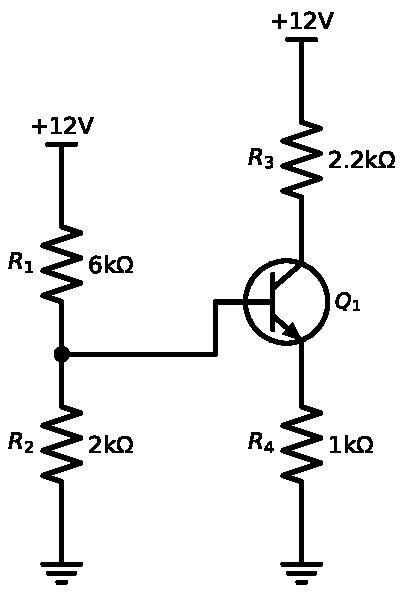
\includegraphics[width=\linewidth,height=7cm,keepaspectratio]{p01_circuit}\end{center}
\end{probbox}

\begin{probbox}{Problem 4A.2 \hfill Easy}
For the circuit below, find the DC collector currents $I_C$ of all transistors and verify all assumptions, including the operating region of every transistor. Assume $\beta = 100$.
\begin{center}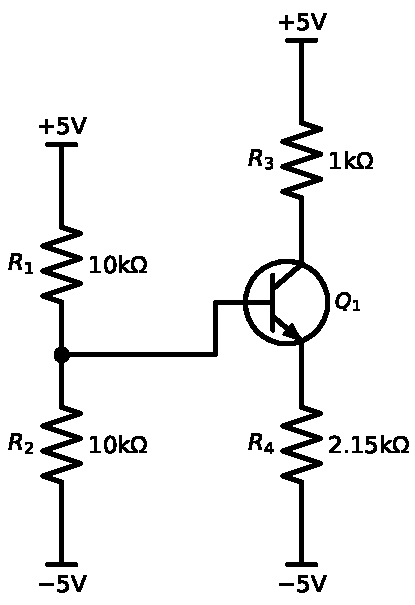
\includegraphics[width=\linewidth,height=7cm,keepaspectratio]{p02_circuit}\end{center}
\end{probbox}

\begin{probbox}{Problem 4A.3 \hfill Easy}
For the circuit below, find the DC collector currents $I_C$ of all transistors and verify all assumptions, including the operating region of every transistor. Assume $\beta = 100$.
\begin{center}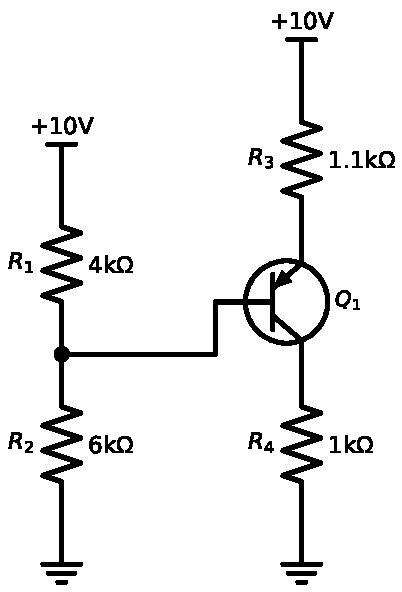
\includegraphics[width=\linewidth,height=7cm,keepaspectratio]{p03_circuit}\end{center}
\end{probbox}

\begin{probbox}{Problem 4A.4 \hfill Easy}
For the circuit below, find the DC collector currents $I_C$ of all transistors and verify all assumptions, including the operating region of every transistor. Assume $\beta = 100$.
\begin{center}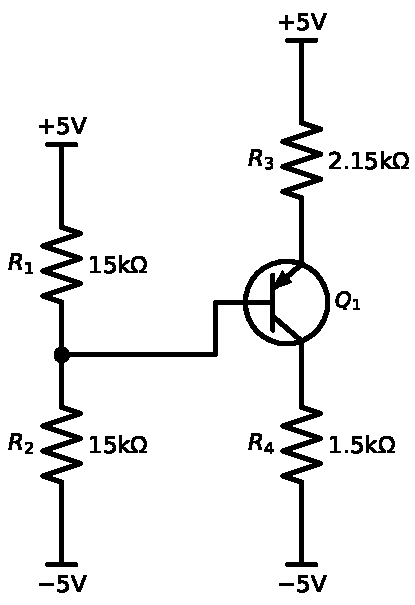
\includegraphics[width=\linewidth,height=7cm,keepaspectratio]{p04_circuit}\end{center}
\end{probbox}

\begin{probbox}{Problem 4A.5 \hfill Easy}
For the circuit below, find the DC collector currents $I_C$ of all transistors and verify all assumptions, including the operating region of every transistor. Assume $\beta = 100$.
\begin{center}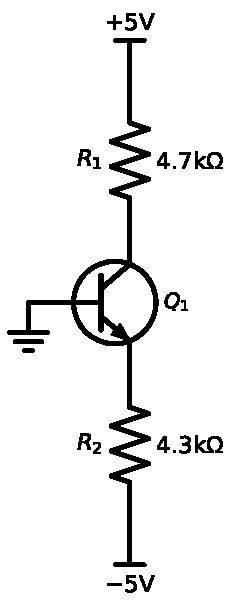
\includegraphics[width=\linewidth,height=7cm,keepaspectratio]{p05_circuit}\end{center}
\end{probbox}

\begin{probbox}{Problem 4A.6 \hfill Easy}
For the circuit below, find the DC collector currents $I_C$ of all transistors and verify all assumptions, including the operating region of every transistor. Assume $\beta = 100$.
\begin{center}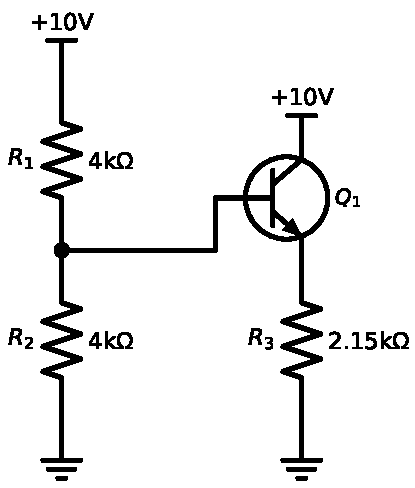
\includegraphics[width=\linewidth,height=7cm,keepaspectratio]{p06_circuit}\end{center}
\end{probbox}

\subsection*{Medium problems}
\begin{probbox}{Problem 4A.7 \hfill Medium}
For the circuit below, find the DC collector currents $I_C$ of all transistors and verify all assumptions, including the operating region of every transistor. Assume $\beta = 100$.
\begin{center}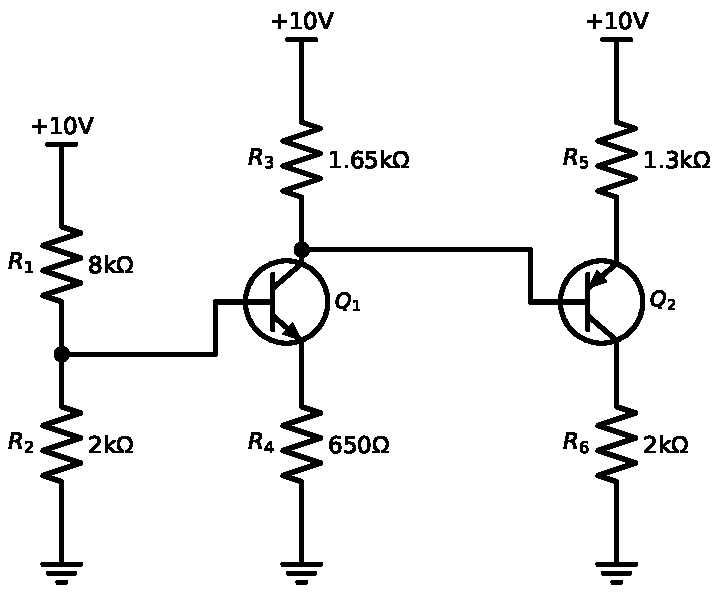
\includegraphics[width=\linewidth,height=7cm,keepaspectratio]{p07_circuit}\end{center}
\end{probbox}

\begin{probbox}{Problem 4A.8 \hfill Medium}
For the circuit below, find the DC collector currents $I_C$ of all transistors and verify all assumptions, including the operating region of every transistor. Assume $\beta = 100$.
\begin{center}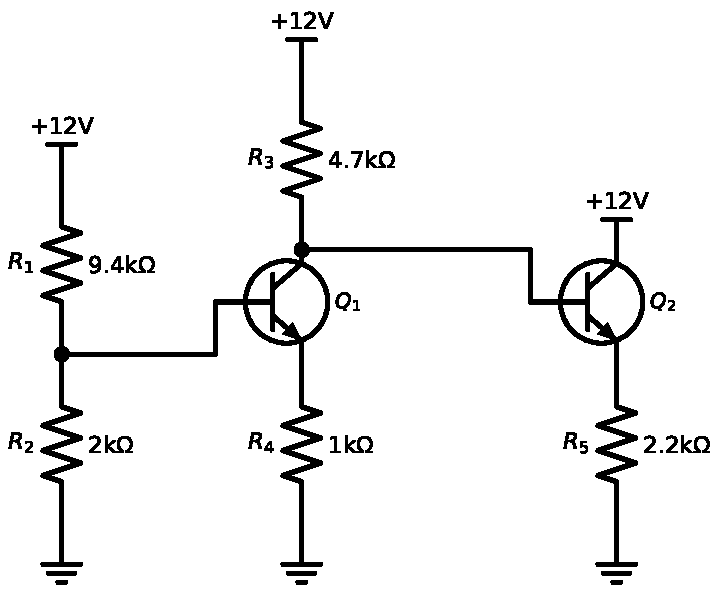
\includegraphics[width=\linewidth,height=7cm,keepaspectratio]{p08_circuit}\end{center}
\end{probbox}

\begin{probbox}{Problem 4A.9 \hfill Medium}
For the circuit below, find the DC collector currents $I_C$ of all transistors and verify all assumptions, including the operating region of every transistor. Assume $\beta = 100$.
\begin{center}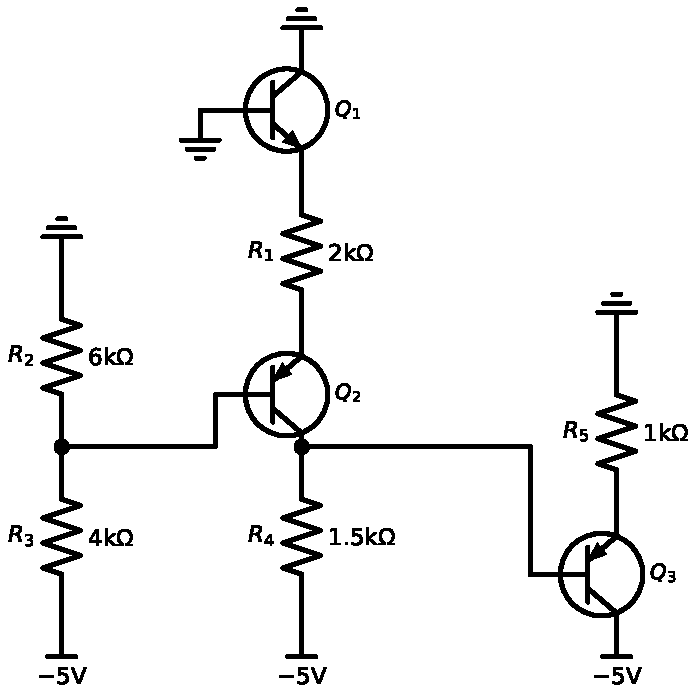
\includegraphics[width=\linewidth,height=7cm,keepaspectratio]{p09_circuit}\end{center}
\end{probbox}

\begin{probbox}{Problem 4A.10 \hfill Medium}
For the circuit below, find the DC collector currents $I_C$ of all transistors and verify all assumptions, including the operating region of every transistor. Assume $\beta = 100$.
\begin{center}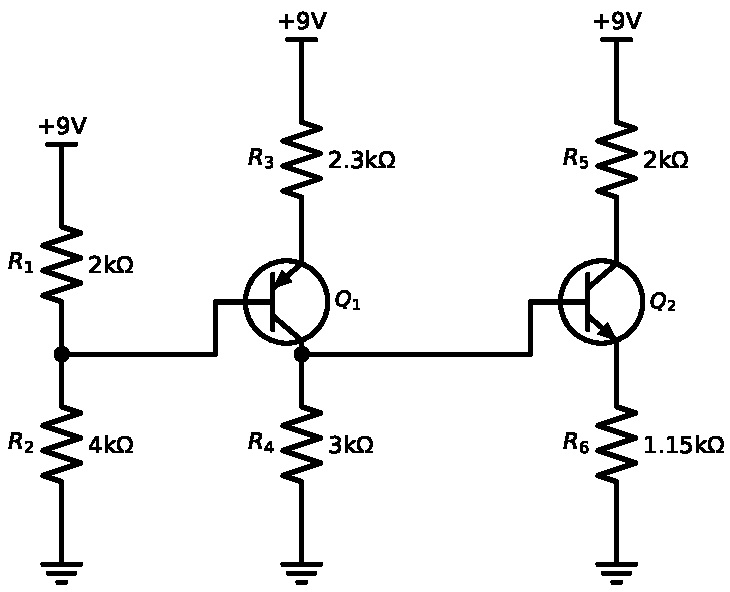
\includegraphics[width=\linewidth,height=7cm,keepaspectratio]{p10_circuit}\end{center}
\end{probbox}

\begin{probbox}{Problem 4A.11 \hfill Medium}
For the circuit below, find the DC collector currents $I_C$ of all transistors and verify all assumptions, including the operating region of every transistor. Assume $\beta = 100$.
\begin{center}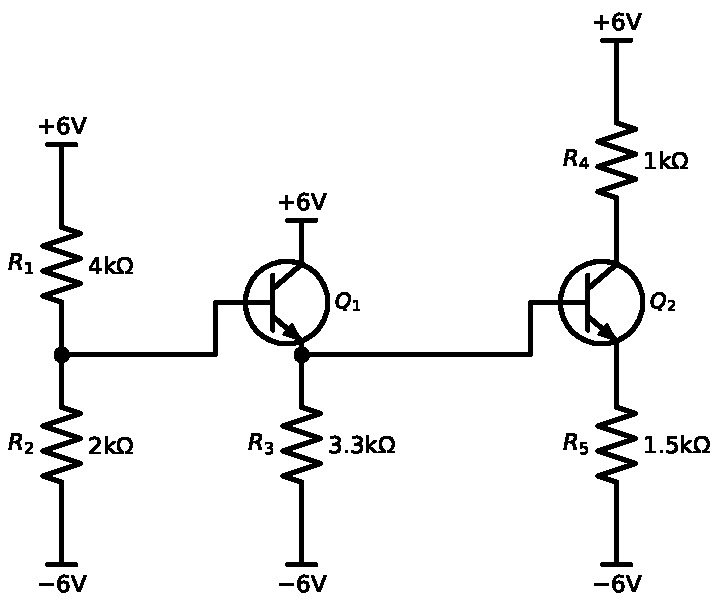
\includegraphics[width=\linewidth,height=7cm,keepaspectratio]{p11_circuit}\end{center}
\end{probbox}

\begin{probbox}{Problem 4A.12 \hfill Medium}
For the circuit below, find the DC collector currents $I_C$ of all transistors and verify all assumptions, including the operating region of every transistor. Assume $\beta = 100$.
\begin{center}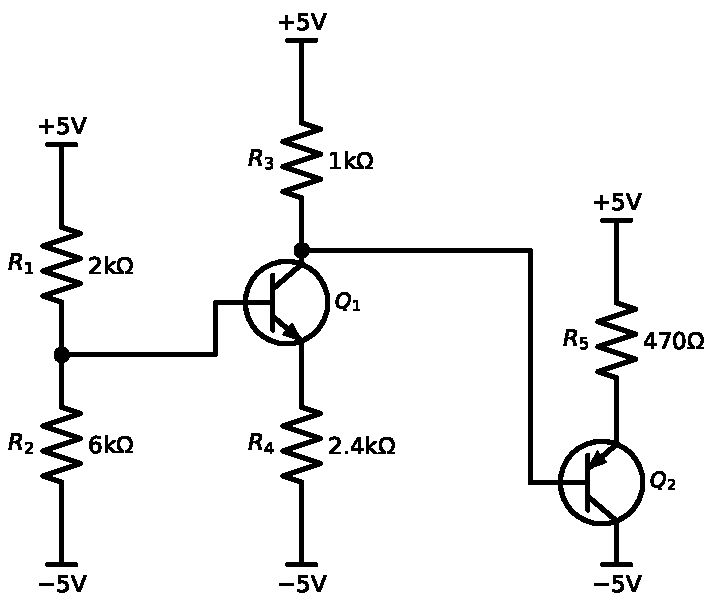
\includegraphics[width=\linewidth,height=7cm,keepaspectratio]{p12_circuit}\end{center}
\end{probbox}

\subsection*{Hard problems}
\begin{probbox}{Problem 4A.13 \hfill Hard}
For the circuit below, find the DC collector currents $I_C$ of all transistors and verify all assumptions, including the operating region of every transistor. Assume $\beta = 100$.
\begin{center}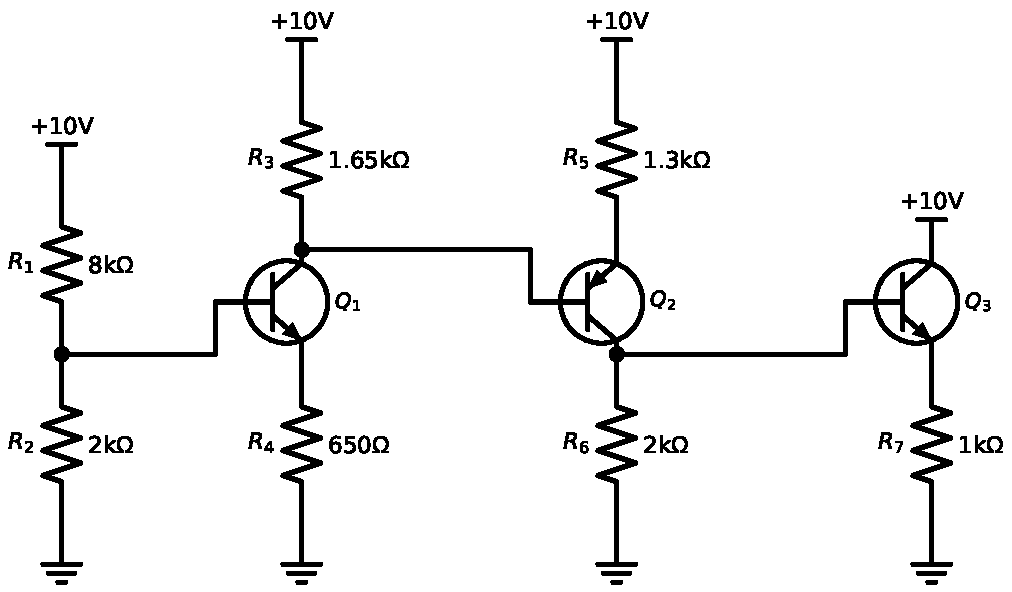
\includegraphics[width=\linewidth,height=7cm,keepaspectratio]{p13_circuit}\end{center}
\end{probbox}

\begin{probbox}{Problem 4A.14 \hfill Hard}
For the circuit below, find the DC collector currents $I_C$ of all transistors and verify all assumptions, including the operating region of every transistor. Assume $\beta = 100$.
\begin{center}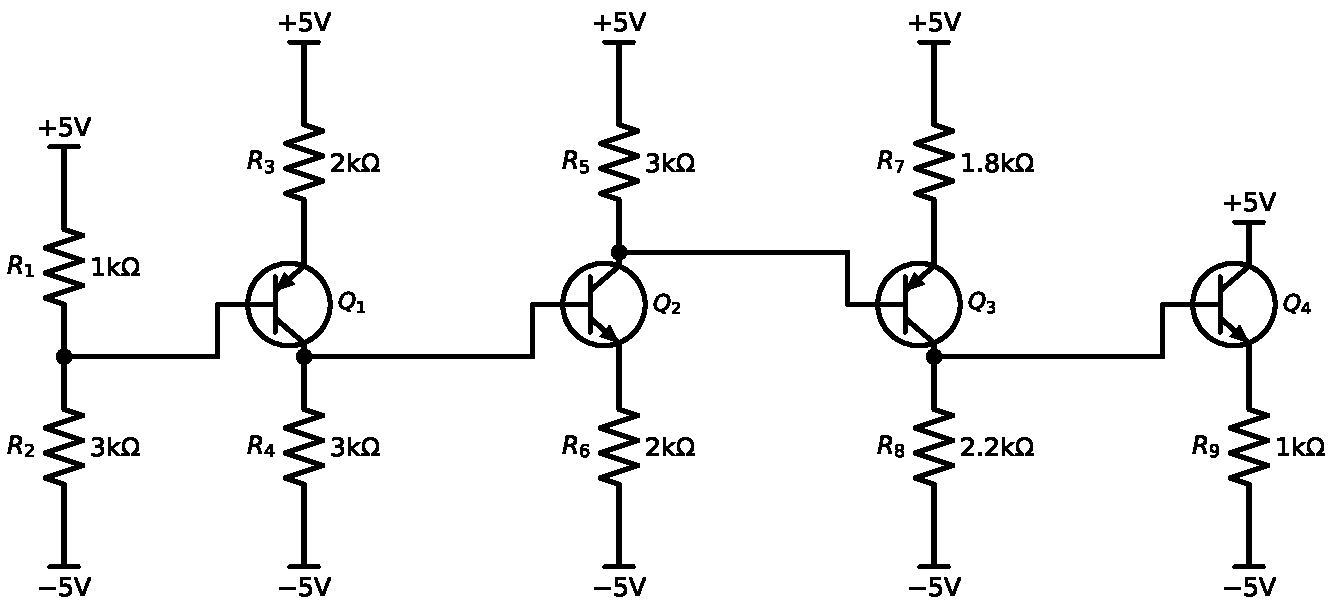
\includegraphics[width=\linewidth,height=7cm,keepaspectratio]{p14_circuit}\end{center}
\end{probbox}

\begin{probbox}{Problem 4A.15 \hfill Hard}
For the circuit below, find the DC collector currents $I_C$ of all transistors and verify all assumptions, including the operating region of every transistor. Assume $\beta = 100$.
\begin{center}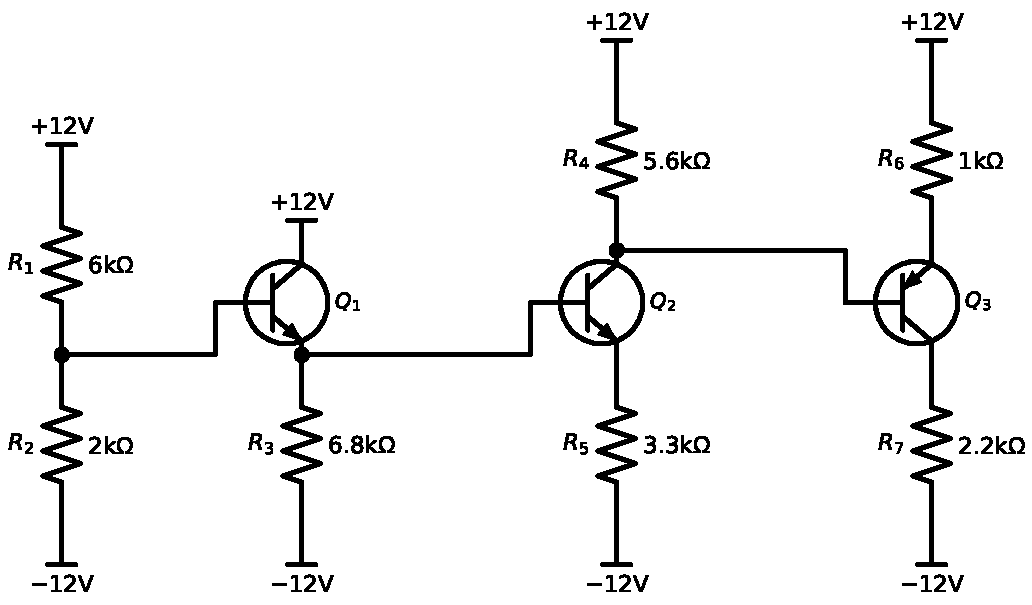
\includegraphics[width=\linewidth,height=7cm,keepaspectratio]{p15_circuit}\end{center}
\end{probbox}

\begin{probbox}{Problem 4A.16 \hfill Hard}
For the circuit below, find the DC collector currents $I_C$ of all transistors and verify all assumptions, including the operating region of every transistor. Assume $\beta = 100$.
\begin{center}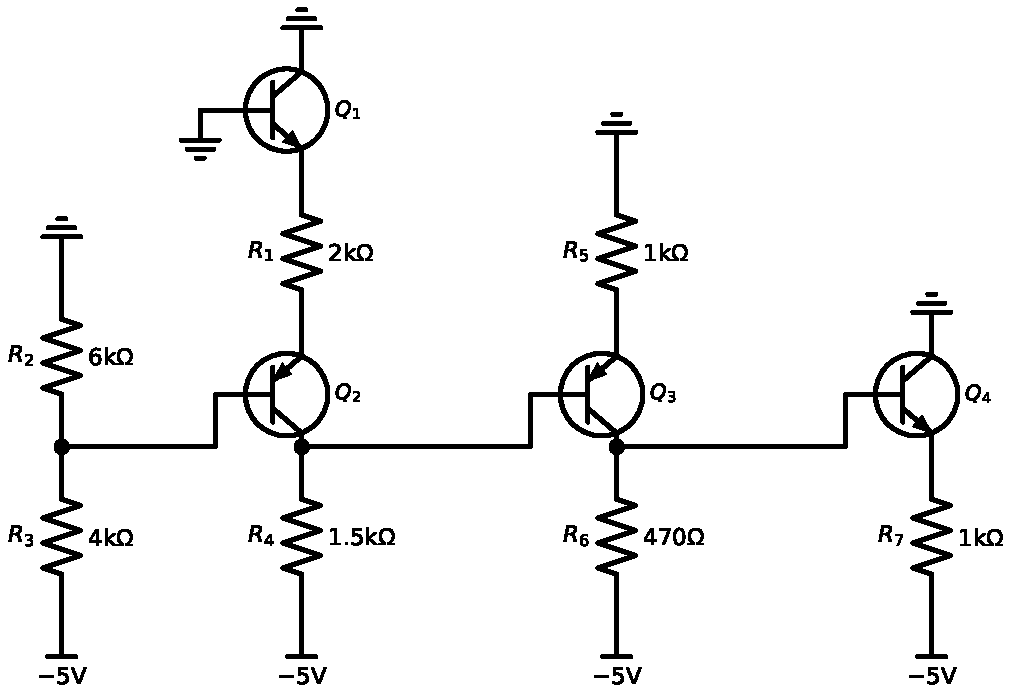
\includegraphics[width=\linewidth,height=7cm,keepaspectratio]{p16_circuit}\end{center}
\end{probbox}

\begin{probbox}{Problem 4A.17 \hfill Hard}
For the circuit below, find the DC collector currents $I_C$ of all transistors and verify all assumptions, including the operating region of every transistor. Assume $\beta = 100$.
\begin{center}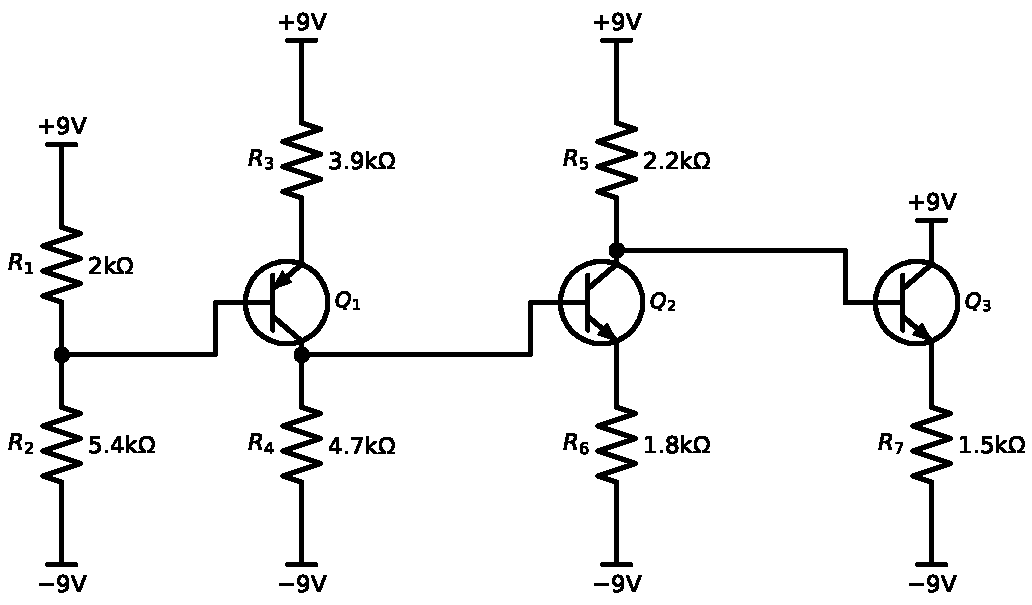
\includegraphics[width=\linewidth,height=7cm,keepaspectratio]{p17_circuit}\end{center}
\end{probbox}

\begin{probbox}{Problem 4A.18 \hfill Hard}
For the circuit below, find the DC collector currents $I_C$ of all transistors and verify all assumptions, including the operating region of every transistor. Assume $\beta = 100$.
\begin{center}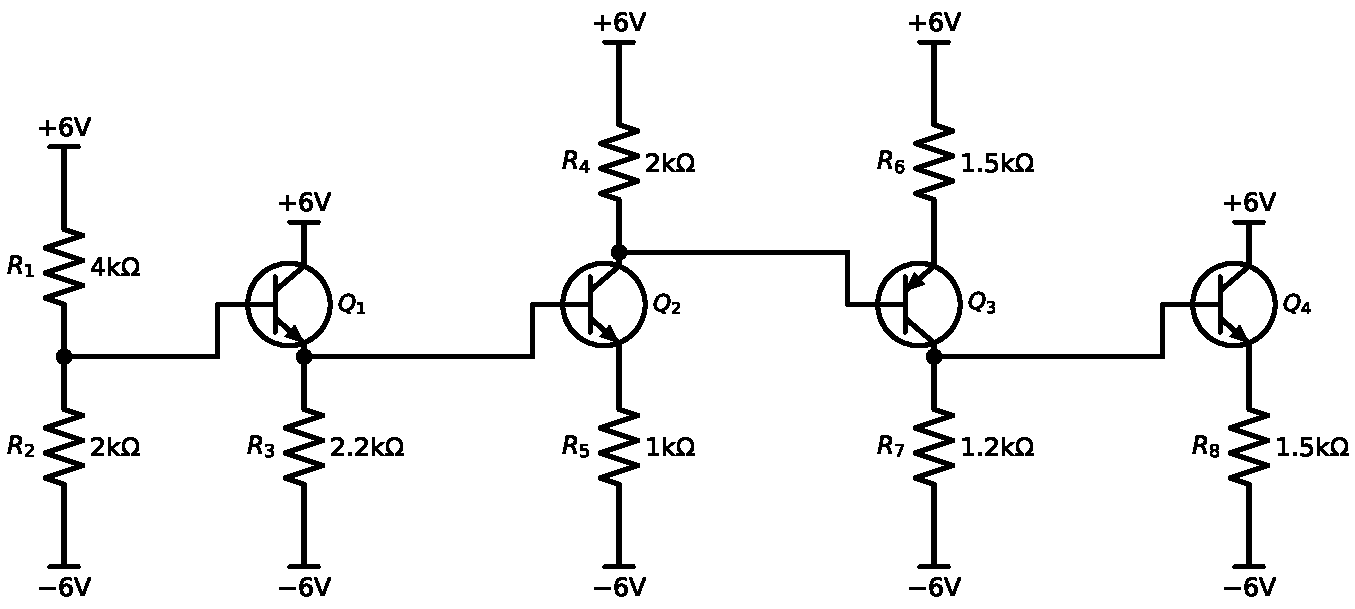
\includegraphics[width=\linewidth,height=7cm,keepaspectratio]{p18_circuit}\end{center}
\end{probbox}

\newpage
\section*{Solutions}
Every solution follows the steps of the Lecture-4 pipeline card.
\subsection*{Solution 4A.1 \hfill Easy}
\begin{center}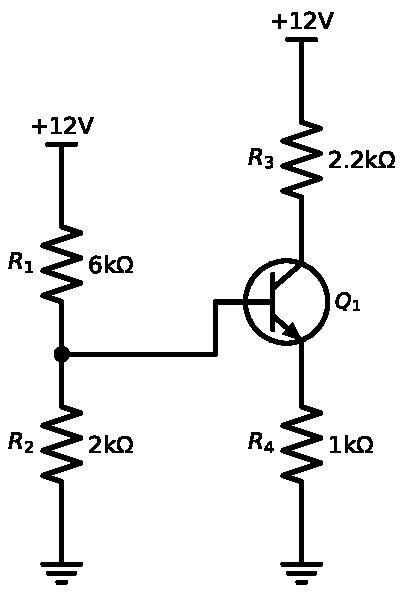
\includegraphics[width=0.9\linewidth,height=6cm,keepaspectratio]{p01_circuit}\end{center}
\solstep{1}{Assumptions}Assume every transistor is in the active region and that every base current is negligible ($I_B\approx0$, tool T1): then $|V_{BE}| = 0.7$\,V, $I_C\approx I_E$, and no current flows into any base, so a base network behaves like a plain resistor divider.
\solstep{2}{Walk through the circuit}\begin{enumerate}[leftmargin=*,itemsep=3pt]
\item No current flows into the base ($I_B$ is negligible), so $V_{B1}$ is set by the divider $R_{1}$--$R_{2}$ between $12$ and $0$ (Lecture-1 tool):\[V_{B1} = 0 + (12 - (0))\frac{2\,\mathrm{k}}{6\,\mathrm{k} + 2\,\mathrm{k}} = 3\,\mathrm{V}\]
\item $Q_{1}$ is npn and assumed active: $V_{BE} = 0.7$\,V, so $V_{E1} = V_{B1} - 0.7 = 2.3\,\mathrm{V}$.
\item KCL at the emitter of $Q_{1}$ (base current neglected): \[I_{E1} = \frac{V_{E1} - 0}{R_{4}} = 2.3\,\mathrm{m}\mathrm{A}, \qquad I_{C1} \approx I_{E1}\]
\item $Q_{1}$ draws $I_{C1} = 2.3\,\mathrm{m}\mathrm{A}$ from $V_{C1}$ through $R_{3}$: $V_{C1} = 12 - R_{3}\,(I_{C1}) = 12 - 2.2\,\mathrm{k}\times2.3\,\mathrm{m}\mathrm{A} = 6.94\,\mathrm{V}$.
\end{enumerate}

\solstep{3}{Verify the assumptions}\begin{itemize}[leftmargin=*,itemsep=2pt]
\item $I_{B1} = \frac{I_{C1}}{\beta} = 23\,\mu \mathrm{A}$ $\ll$ the $1.5\,\mathrm{m}\mathrm{A}$ flowing in the base network \checkmark
\item $V_{CE1} = V_{C1} - V_{E1} = 6.94 - (2.3) = 4.64\,\mathrm{V}$ $\ge 0.2$\,V $\Rightarrow$ $Q_{1}$ is active \checkmark
\end{itemize}

\solstep{4}{How good was $I_B\approx 0$?}If we keep the base currents ($I_C=\beta I_B$ with $\beta=100$) and solve the circuit exactly, the currents change only a little:\begin{center}\renewcommand{\arraystretch}{1.35}
\begin{tabular}{cccc}
\toprule
transistor & $I_C$ (with $I_B\approx0$) & $I_C$ (exact) & difference \\
\midrule
$Q_{1}$ & $2.3\,\mathrm{m}\mathrm{A}$ & $2.24\,\mathrm{m}\mathrm{A}$ & $2.5\%$ \\
\bottomrule
\end{tabular}\end{center}

\begin{ansbox}
$I_{C1} = 2.3\,\mathrm{m}\mathrm{A}$\\[2pt] all transistors active, all base currents negligible.
\end{ansbox}

\newpage
\subsection*{Solution 4A.2 \hfill Easy}
\begin{center}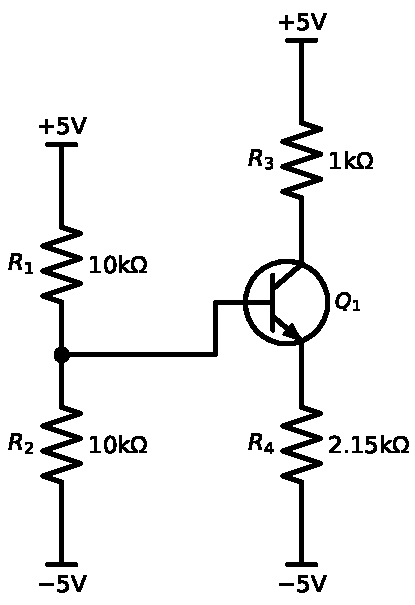
\includegraphics[width=0.9\linewidth,height=6cm,keepaspectratio]{p02_circuit}\end{center}
\solstep{1}{Assumptions}Assume every transistor is in the active region and that every base current is negligible ($I_B\approx0$, tool T1): then $|V_{BE}| = 0.7$\,V, $I_C\approx I_E$, and no current flows into any base, so a base network behaves like a plain resistor divider.
\solstep{2}{Walk through the circuit}\begin{enumerate}[leftmargin=*,itemsep=3pt]
\item No current flows into the base ($I_B$ is negligible), so $V_{B1}$ is set by the divider $R_{1}$--$R_{2}$ between $5$ and $(-5)$ (Lecture-1 tool):\[V_{B1} = -5 + (5 - (-5))\frac{10\,\mathrm{k}}{10\,\mathrm{k} + 10\,\mathrm{k}} = 0\,\mathrm{V}\]
\item $Q_{1}$ is npn and assumed active: $V_{BE} = 0.7$\,V, so $V_{E1} = V_{B1} - 0.7 = -0.7\,\mathrm{V}$.
\item KCL at the emitter of $Q_{1}$ (base current neglected): \[I_{E1} = \frac{V_{E1} - (-5)}{R_{4}} = 2\,\mathrm{m}\mathrm{A}, \qquad I_{C1} \approx I_{E1}\]
\item $Q_{1}$ draws $I_{C1} = 2\,\mathrm{m}\mathrm{A}$ from $V_{C1}$ through $R_{3}$: $V_{C1} = 5 - R_{3}\,(I_{C1}) = 5 - 1\,\mathrm{k}\times2\,\mathrm{m}\mathrm{A} = 3\,\mathrm{V}$.
\end{enumerate}

\solstep{3}{Verify the assumptions}\begin{itemize}[leftmargin=*,itemsep=2pt]
\item $I_{B1} = \frac{I_{C1}}{\beta} = 20\,\mu \mathrm{A}$ $\ll$ the $500\,\mu \mathrm{A}$ flowing in the base network \checkmark
\item $V_{CE1} = V_{C1} - V_{E1} = 3 - (-0.7) = 3.7\,\mathrm{V}$ $\ge 0.2$\,V $\Rightarrow$ $Q_{1}$ is active \checkmark
\end{itemize}

\solstep{4}{How good was $I_B\approx 0$?}If we keep the base currents ($I_C=\beta I_B$ with $\beta=100$) and solve the circuit exactly, the currents change only a little:\begin{center}\renewcommand{\arraystretch}{1.35}
\begin{tabular}{cccc}
\toprule
transistor & $I_C$ (with $I_B\approx0$) & $I_C$ (exact) & difference \\
\midrule
$Q_{1}$ & $2\,\mathrm{m}\mathrm{A}$ & $1.94\,\mathrm{m}\mathrm{A}$ & $3.3\%$ \\
\bottomrule
\end{tabular}\end{center}

\begin{ansbox}
$I_{C1} = 2\,\mathrm{m}\mathrm{A}$\\[2pt] all transistors active, all base currents negligible.
\end{ansbox}

\newpage
\subsection*{Solution 4A.3 \hfill Easy}
\begin{center}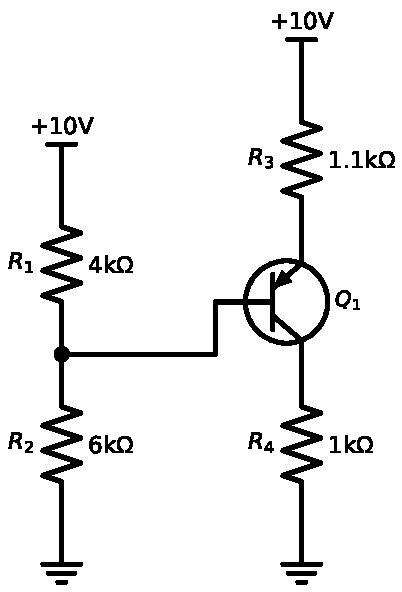
\includegraphics[width=0.9\linewidth,height=6cm,keepaspectratio]{p03_circuit}\end{center}
\solstep{1}{Assumptions}Assume every transistor is in the active region and that every base current is negligible ($I_B\approx0$, tool T1): then $|V_{BE}| = 0.7$\,V, $I_C\approx I_E$, and no current flows into any base, so a base network behaves like a plain resistor divider.
\solstep{2}{Walk through the circuit}\begin{enumerate}[leftmargin=*,itemsep=3pt]
\item No current flows into the base ($I_B$ is negligible), so $V_{B1}$ is set by the divider $R_{1}$--$R_{2}$ between $10$ and $0$ (Lecture-1 tool):\[V_{B1} = 0 + (10 - (0))\frac{6\,\mathrm{k}}{4\,\mathrm{k} + 6\,\mathrm{k}} = 6\,\mathrm{V}\]
\item $Q_{1}$ is pnp and assumed active: $V_{BE} = -0.7$\,V, so $V_{E1} = V_{B1} + 0.7 = 6.7\,\mathrm{V}$.
\item KCL at the emitter of $Q_{1}$ (base current neglected): \[I_{E1} = \frac{10 - V_{E1}}{R_{3}} = 3\,\mathrm{m}\mathrm{A}, \qquad I_{C1} \approx I_{E1}\]
\item The current $I_{C1} = 3\,\mathrm{m}\mathrm{A}$ flows from $V_{C1}$ through $R_{4}$: $V_{C1} = 0 + R_{4}\,(I_{C1}) = 0 + 1\,\mathrm{k}\times3\,\mathrm{m}\mathrm{A} = 3\,\mathrm{V}$.
\end{enumerate}

\solstep{3}{Verify the assumptions}\begin{itemize}[leftmargin=*,itemsep=2pt]
\item $I_{B1} = \frac{I_{C1}}{\beta} = 30\,\mu \mathrm{A}$ $\ll$ the $1\,\mathrm{m}\mathrm{A}$ flowing in the base network \checkmark
\item $V_{EC1} = V_{E1} - V_{C1} = 6.7 - (3) = 3.7\,\mathrm{V}$ $\ge 0.2$\,V $\Rightarrow$ $Q_{1}$ is active \checkmark
\end{itemize}

\solstep{4}{How good was $I_B\approx 0$?}If we keep the base currents ($I_C=\beta I_B$ with $\beta=100$) and solve the circuit exactly, the currents change only a little:\begin{center}\renewcommand{\arraystretch}{1.35}
\begin{tabular}{cccc}
\toprule
transistor & $I_C$ (with $I_B\approx0$) & $I_C$ (exact) & difference \\
\midrule
$Q_{1}$ & $3\,\mathrm{m}\mathrm{A}$ & $2.91\,\mathrm{m}\mathrm{A}$ & $3.2\%$ \\
\bottomrule
\end{tabular}\end{center}

\begin{ansbox}
$I_{C1} = 3\,\mathrm{m}\mathrm{A}$\\[2pt] all transistors active, all base currents negligible.
\end{ansbox}

\newpage
\subsection*{Solution 4A.4 \hfill Easy}
\begin{center}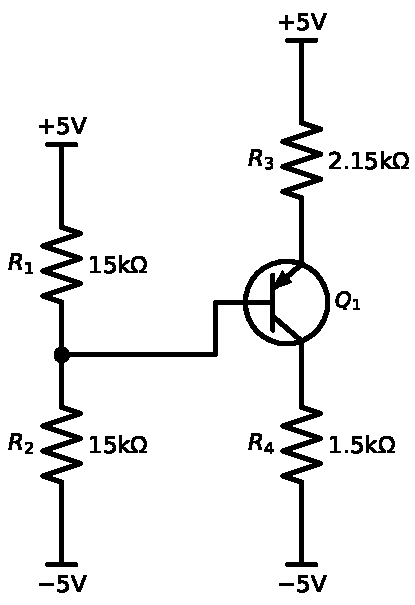
\includegraphics[width=0.9\linewidth,height=6cm,keepaspectratio]{p04_circuit}\end{center}
\solstep{1}{Assumptions}Assume every transistor is in the active region and that every base current is negligible ($I_B\approx0$, tool T1): then $|V_{BE}| = 0.7$\,V, $I_C\approx I_E$, and no current flows into any base, so a base network behaves like a plain resistor divider.
\solstep{2}{Walk through the circuit}\begin{enumerate}[leftmargin=*,itemsep=3pt]
\item No current flows into the base ($I_B$ is negligible), so $V_{B1}$ is set by the divider $R_{1}$--$R_{2}$ between $5$ and $(-5)$ (Lecture-1 tool):\[V_{B1} = -5 + (5 - (-5))\frac{15\,\mathrm{k}}{15\,\mathrm{k} + 15\,\mathrm{k}} = 0\,\mathrm{V}\]
\item $Q_{1}$ is pnp and assumed active: $V_{BE} = -0.7$\,V, so $V_{E1} = V_{B1} + 0.7 = 0.7\,\mathrm{V}$.
\item KCL at the emitter of $Q_{1}$ (base current neglected): \[I_{E1} = \frac{5 - V_{E1}}{R_{3}} = 2\,\mathrm{m}\mathrm{A}, \qquad I_{C1} \approx I_{E1}\]
\item The current $I_{C1} = 2\,\mathrm{m}\mathrm{A}$ flows from $V_{C1}$ through $R_{4}$: $V_{C1} = (-5) + R_{4}\,(I_{C1}) = -5 + 1.5\,\mathrm{k}\times2\,\mathrm{m}\mathrm{A} = -2\,\mathrm{V}$.
\end{enumerate}

\solstep{3}{Verify the assumptions}\begin{itemize}[leftmargin=*,itemsep=2pt]
\item $I_{B1} = \frac{I_{C1}}{\beta} = 20\,\mu \mathrm{A}$ $\ll$ the $333\,\mu \mathrm{A}$ flowing in the base network \checkmark
\item $V_{EC1} = V_{E1} - V_{C1} = 0.7 - (-2) = 2.7\,\mathrm{V}$ $\ge 0.2$\,V $\Rightarrow$ $Q_{1}$ is active \checkmark
\end{itemize}

\solstep{4}{How good was $I_B\approx 0$?}If we keep the base currents ($I_C=\beta I_B$ with $\beta=100$) and solve the circuit exactly, the currents change only a little:\begin{center}\renewcommand{\arraystretch}{1.35}
\begin{tabular}{cccc}
\toprule
transistor & $I_C$ (with $I_B\approx0$) & $I_C$ (exact) & difference \\
\midrule
$Q_{1}$ & $2\,\mathrm{m}\mathrm{A}$ & $1.91\,\mathrm{m}\mathrm{A}$ & $4.5\%$ \\
\bottomrule
\end{tabular}\end{center}

\begin{ansbox}
$I_{C1} = 2\,\mathrm{m}\mathrm{A}$\\[2pt] all transistors active, all base currents negligible.
\end{ansbox}

\newpage
\subsection*{Solution 4A.5 \hfill Easy}
\begin{center}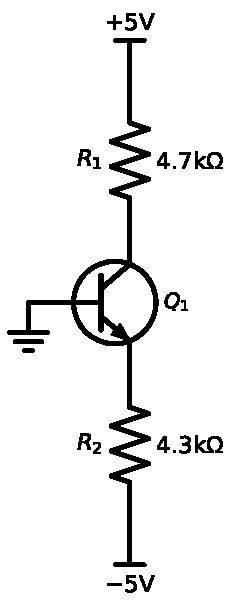
\includegraphics[width=0.9\linewidth,height=6cm,keepaspectratio]{p05_circuit}\end{center}
\solstep{1}{Assumptions}Assume every transistor is in the active region and that every base current is negligible ($I_B\approx0$, tool T1): then $|V_{BE}| = 0.7$\,V, $I_C\approx I_E$, and no current flows into any base, so a base network behaves like a plain resistor divider.
\solstep{2}{Walk through the circuit}\begin{enumerate}[leftmargin=*,itemsep=3pt]
\item $Q_{1}$ is npn and assumed active: $V_{BE} = 0.7$\,V, so $V_{E1} = 0 - 0.7 = -0.7\,\mathrm{V}$.
\item KCL at the emitter of $Q_{1}$ (base current neglected): \[I_{E1} = \frac{V_{E1} - (-5)}{R_{2}} = 1\,\mathrm{m}\mathrm{A}, \qquad I_{C1} \approx I_{E1}\]
\item $Q_{1}$ draws $I_{C1} = 1\,\mathrm{m}\mathrm{A}$ from $V_{C1}$ through $R_{1}$: $V_{C1} = 5 - R_{1}\,(I_{C1}) = 5 - 4.7\,\mathrm{k}\times1\,\mathrm{m}\mathrm{A} = 0.3\,\mathrm{V}$.
\end{enumerate}

\solstep{3}{Verify the assumptions}\begin{itemize}[leftmargin=*,itemsep=2pt]
\item $V_{CE1} = V_{C1} - V_{E1} = 0.3 - (-0.7) = 1\,\mathrm{V}$ $\ge 0.2$\,V $\Rightarrow$ $Q_{1}$ is active \checkmark
\end{itemize}

\solstep{4}{How good was $I_B\approx 0$?}If we keep the base currents ($I_C=\beta I_B$ with $\beta=100$) and solve the circuit exactly, the currents change only a little:\begin{center}\renewcommand{\arraystretch}{1.35}
\begin{tabular}{cccc}
\toprule
transistor & $I_C$ (with $I_B\approx0$) & $I_C$ (exact) & difference \\
\midrule
$Q_{1}$ & $1\,\mathrm{m}\mathrm{A}$ & $990\,\mu \mathrm{A}$ & $1\%$ \\
\bottomrule
\end{tabular}\end{center}

\begin{ansbox}
$I_{C1} = 1\,\mathrm{m}\mathrm{A}$\\[2pt] all transistors active, all base currents negligible.
\end{ansbox}

\newpage
\subsection*{Solution 4A.6 \hfill Easy}
\begin{center}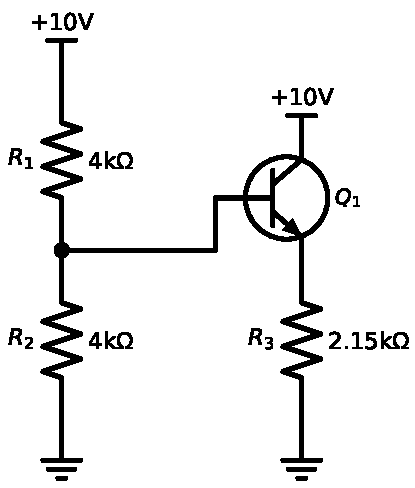
\includegraphics[width=0.9\linewidth,height=6cm,keepaspectratio]{p06_circuit}\end{center}
\solstep{1}{Assumptions}Assume every transistor is in the active region and that every base current is negligible ($I_B\approx0$, tool T1): then $|V_{BE}| = 0.7$\,V, $I_C\approx I_E$, and no current flows into any base, so a base network behaves like a plain resistor divider.
\solstep{2}{Walk through the circuit}\begin{enumerate}[leftmargin=*,itemsep=3pt]
\item No current flows into the base ($I_B$ is negligible), so $V_{B1}$ is set by the divider $R_{1}$--$R_{2}$ between $10$ and $0$ (Lecture-1 tool):\[V_{B1} = 0 + (10 - (0))\frac{4\,\mathrm{k}}{4\,\mathrm{k} + 4\,\mathrm{k}} = 5\,\mathrm{V}\]
\item $Q_{1}$ is npn and assumed active: $V_{BE} = 0.7$\,V, so $V_{E1} = V_{B1} - 0.7 = 4.3\,\mathrm{V}$.
\item KCL at the emitter of $Q_{1}$ (base current neglected): \[I_{E1} = \frac{V_{E1} - 0}{R_{3}} = 2\,\mathrm{m}\mathrm{A}, \qquad I_{C1} \approx I_{E1}\]
\end{enumerate}

\solstep{3}{Verify the assumptions}\begin{itemize}[leftmargin=*,itemsep=2pt]
\item $I_{B1} = \frac{I_{C1}}{\beta} = 20\,\mu \mathrm{A}$ $\ll$ the $1.25\,\mathrm{m}\mathrm{A}$ flowing in the base network \checkmark
\item $V_{CE1} = 10 - V_{E1} = 10 - (4.3) = 5.7\,\mathrm{V}$ $\ge 0.2$\,V $\Rightarrow$ $Q_{1}$ is active \checkmark
\end{itemize}

\solstep{4}{How good was $I_B\approx 0$?}If we keep the base currents ($I_C=\beta I_B$ with $\beta=100$) and solve the circuit exactly, the currents change only a little:\begin{center}\renewcommand{\arraystretch}{1.35}
\begin{tabular}{cccc}
\toprule
transistor & $I_C$ (with $I_B\approx0$) & $I_C$ (exact) & difference \\
\midrule
$Q_{1}$ & $2\,\mathrm{m}\mathrm{A}$ & $1.96\,\mathrm{m}\mathrm{A}$ & $1.9\%$ \\
\bottomrule
\end{tabular}\end{center}

\begin{ansbox}
$I_{C1} = 2\,\mathrm{m}\mathrm{A}$\\[2pt] all transistors active, all base currents negligible.
\end{ansbox}

\newpage
\subsection*{Solution 4A.7 \hfill Medium}
\begin{center}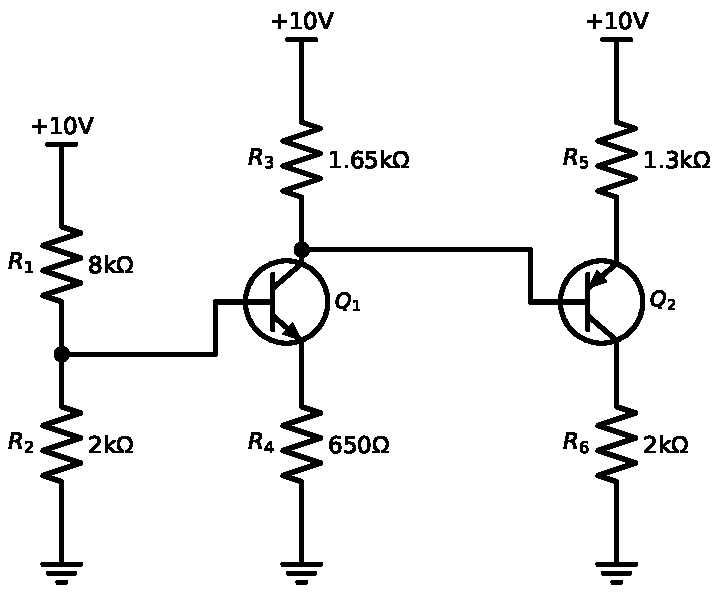
\includegraphics[width=0.9\linewidth,height=6cm,keepaspectratio]{p07_circuit}\end{center}
\solstep{1}{Assumptions}Assume every transistor is in the active region and that every base current is negligible ($I_B\approx0$, tool T1): then $|V_{BE}| = 0.7$\,V, $I_C\approx I_E$, and no current flows into any base, so a base network behaves like a plain resistor divider.
\solstep{2}{Walk through the circuit}\begin{enumerate}[leftmargin=*,itemsep=3pt]
\item No current flows into the base ($I_B$ is negligible), so $V_{B1}$ is set by the divider $R_{1}$--$R_{2}$ between $10$ and $0$ (Lecture-1 tool):\[V_{B1} = 0 + (10 - (0))\frac{2\,\mathrm{k}}{8\,\mathrm{k} + 2\,\mathrm{k}} = 2\,\mathrm{V}\]
\item $Q_{1}$ is npn and assumed active: $V_{BE} = 0.7$\,V, so $V_{E1} = V_{B1} - 0.7 = 1.3\,\mathrm{V}$.
\item KCL at the emitter of $Q_{1}$ (base current neglected): \[I_{E1} = \frac{V_{E1} - 0}{R_{4}} = 2\,\mathrm{m}\mathrm{A}, \qquad I_{C1} \approx I_{E1}\]
\item $Q_{1}$ draws $I_{C1} = 2\,\mathrm{m}\mathrm{A}$ from $V_{C1}$ through $R_{3}$: $V_{C1} = 10 - R_{3}\,(I_{C1}) = 10 - 1.65\,\mathrm{k}\times2\,\mathrm{m}\mathrm{A} = 6.7\,\mathrm{V}$.
\item $Q_{2}$ is pnp and assumed active: $V_{BE} = -0.7$\,V, so $V_{E2} = V_{C1} + 0.7 = 7.4\,\mathrm{V}$.
\item KCL at the emitter of $Q_{2}$ (base current neglected): \[I_{E2} = \frac{10 - V_{E2}}{R_{5}} = 2\,\mathrm{m}\mathrm{A}, \qquad I_{C2} \approx I_{E2}\]
\item The current $I_{C2} = 2\,\mathrm{m}\mathrm{A}$ flows from $V_{C2}$ through $R_{6}$: $V_{C2} = 0 + R_{6}\,(I_{C2}) = 0 + 2\,\mathrm{k}\times2\,\mathrm{m}\mathrm{A} = 4\,\mathrm{V}$.
\end{enumerate}

\solstep{3}{Verify the assumptions}\begin{itemize}[leftmargin=*,itemsep=2pt]
\item $I_{B1} = \frac{I_{C1}}{\beta} = 20\,\mu \mathrm{A}$ $\ll$ the $1\,\mathrm{m}\mathrm{A}$ flowing in the base network \checkmark
\item $I_{B2} = \frac{I_{C2}}{\beta} = 20\,\mu \mathrm{A}$ $\ll$ the $2\,\mathrm{m}\mathrm{A}$ flowing in the base network \checkmark
\item $V_{CE1} = V_{C1} - V_{E1} = 6.7 - (1.3) = 5.4\,\mathrm{V}$ $\ge 0.2$\,V $\Rightarrow$ $Q_{1}$ is active \checkmark
\item $V_{EC2} = V_{E2} - V_{C2} = 7.4 - (4) = 3.4\,\mathrm{V}$ $\ge 0.2$\,V $\Rightarrow$ $Q_{2}$ is active \checkmark
\end{itemize}

\solstep{4}{How good was $I_B\approx 0$?}If we keep the base currents ($I_C=\beta I_B$ with $\beta=100$) and solve the circuit exactly, the currents change only a little:\begin{center}\renewcommand{\arraystretch}{1.35}
\begin{tabular}{cccc}
\toprule
transistor & $I_C$ (with $I_B\approx0$) & $I_C$ (exact) & difference \\
\midrule
$Q_{1}$ & $2\,\mathrm{m}\mathrm{A}$ & $1.93\,\mathrm{m}\mathrm{A}$ & $3.5\%$ \\
$Q_{2}$ & $2\,\mathrm{m}\mathrm{A}$ & $1.87\,\mathrm{m}\mathrm{A}$ & $6.8\%$ \\
\bottomrule
\end{tabular}\end{center}
 The differences grow along the chain: every base current slightly shifts the collector voltage that biases the next transistor, and $\alpha = \beta/(\beta+1)$ makes each $I_C$ about 1\,\% smaller than its $I_E$. A shift is amplified when the next stage has only a small voltage across its emitter resistor. Hand analysis with $I_B\approx0$ is still the standard first pass.
\begin{ansbox}
$I_{C1} = 2\,\mathrm{m}\mathrm{A}$,\quad $I_{C2} = 2\,\mathrm{m}\mathrm{A}$\\[2pt] all transistors active, all base currents negligible.
\end{ansbox}

\newpage
\subsection*{Solution 4A.8 \hfill Medium}
\begin{center}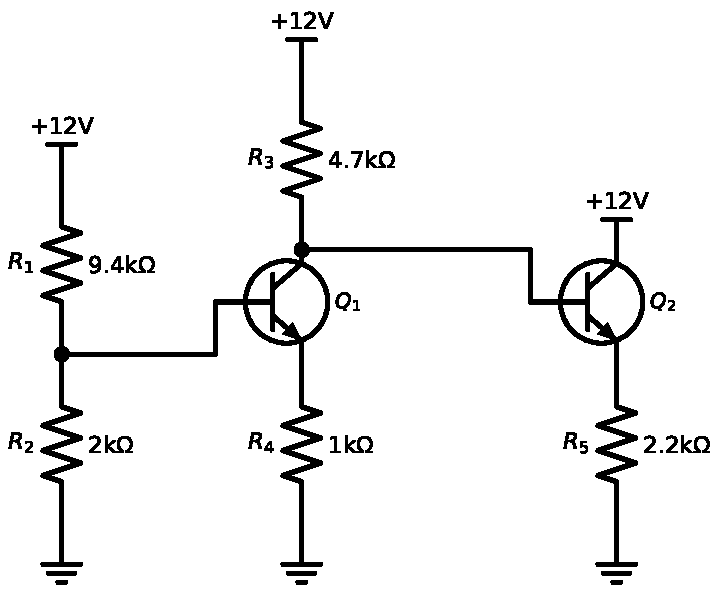
\includegraphics[width=0.9\linewidth,height=6cm,keepaspectratio]{p08_circuit}\end{center}
\solstep{1}{Assumptions}Assume every transistor is in the active region and that every base current is negligible ($I_B\approx0$, tool T1): then $|V_{BE}| = 0.7$\,V, $I_C\approx I_E$, and no current flows into any base, so a base network behaves like a plain resistor divider.
\solstep{2}{Walk through the circuit}\begin{enumerate}[leftmargin=*,itemsep=3pt]
\item No current flows into the base ($I_B$ is negligible), so $V_{B1}$ is set by the divider $R_{1}$--$R_{2}$ between $12$ and $0$ (Lecture-1 tool):\[V_{B1} = 0 + (12 - (0))\frac{2\,\mathrm{k}}{9.4\,\mathrm{k} + 2\,\mathrm{k}} = 2.11\,\mathrm{V}\]
\item $Q_{1}$ is npn and assumed active: $V_{BE} = 0.7$\,V, so $V_{E1} = V_{B1} - 0.7 = 1.41\,\mathrm{V}$.
\item KCL at the emitter of $Q_{1}$ (base current neglected): \[I_{E1} = \frac{V_{E1} - 0}{R_{4}} = 1.41\,\mathrm{m}\mathrm{A}, \qquad I_{C1} \approx I_{E1}\]
\item $Q_{1}$ draws $I_{C1} = 1.41\,\mathrm{m}\mathrm{A}$ from $V_{C1}$ through $R_{3}$: $V_{C1} = 12 - R_{3}\,(I_{C1}) = 12 - 4.7\,\mathrm{k}\times1.41\,\mathrm{m}\mathrm{A} = 5.4\,\mathrm{V}$.
\item $Q_{2}$ is npn and assumed active: $V_{BE} = 0.7$\,V, so $V_{E2} = V_{C1} - 0.7 = 4.7\,\mathrm{V}$.
\item KCL at the emitter of $Q_{2}$ (base current neglected): \[I_{E2} = \frac{V_{E2} - 0}{R_{5}} = 2.13\,\mathrm{m}\mathrm{A}, \qquad I_{C2} \approx I_{E2}\]
\end{enumerate}

\solstep{3}{Verify the assumptions}\begin{itemize}[leftmargin=*,itemsep=2pt]
\item $I_{B1} = \frac{I_{C1}}{\beta} = 14.1\,\mu \mathrm{A}$ $\ll$ the $1.05\,\mathrm{m}\mathrm{A}$ flowing in the base network \checkmark
\item $I_{B2} = \frac{I_{C2}}{\beta} = 21.3\,\mu \mathrm{A}$ $\ll$ the $1.41\,\mathrm{m}\mathrm{A}$ flowing in the base network \checkmark
\item $V_{CE1} = V_{C1} - V_{E1} = 5.395 - (1.405) = 3.99\,\mathrm{V}$ $\ge 0.2$\,V $\Rightarrow$ $Q_{1}$ is active \checkmark
\item $V_{CE2} = 12 - V_{E2} = 12 - (4.695) = 7.3\,\mathrm{V}$ $\ge 0.2$\,V $\Rightarrow$ $Q_{2}$ is active \checkmark
\end{itemize}

\solstep{4}{How good was $I_B\approx 0$?}If we keep the base currents ($I_C=\beta I_B$ with $\beta=100$) and solve the circuit exactly, the currents change only a little:\begin{center}\renewcommand{\arraystretch}{1.35}
\begin{tabular}{cccc}
\toprule
transistor & $I_C$ (with $I_B\approx0$) & $I_C$ (exact) & difference \\
\midrule
$Q_{1}$ & $1.41\,\mathrm{m}\mathrm{A}$ & $1.37\,\mathrm{m}\mathrm{A}$ & $2.6\%$ \\
$Q_{2}$ & $2.13\,\mathrm{m}\mathrm{A}$ & $2.14\,\mathrm{m}\mathrm{A}$ & $-0.48\%$ \\
\bottomrule
\end{tabular}\end{center}

\begin{ansbox}
$I_{C1} = 1.41\,\mathrm{m}\mathrm{A}$,\quad $I_{C2} = 2.13\,\mathrm{m}\mathrm{A}$\\[2pt] all transistors active, all base currents negligible.
\end{ansbox}

\newpage
\subsection*{Solution 4A.9 \hfill Medium}
\begin{center}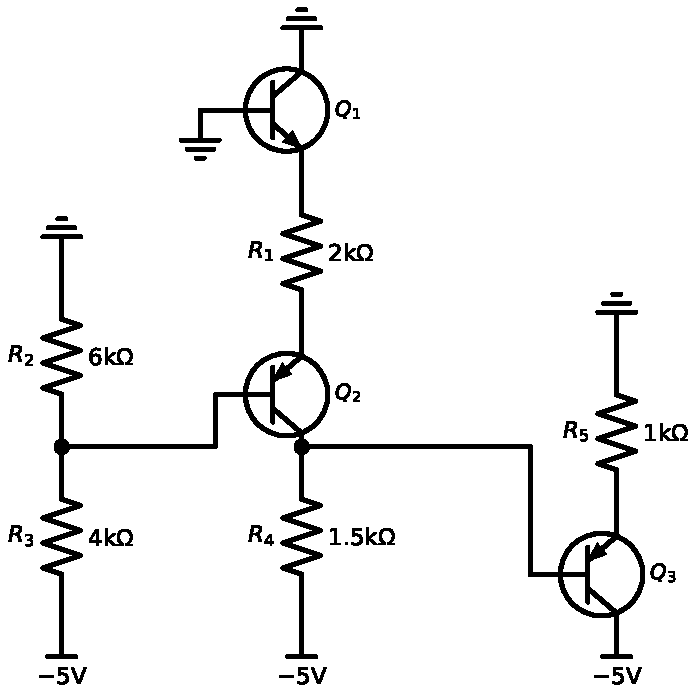
\includegraphics[width=0.9\linewidth,height=6cm,keepaspectratio]{p09_circuit}\end{center}
\solstep{1}{Assumptions}Assume every transistor is in the active region and that every base current is negligible ($I_B\approx0$, tool T1): then $|V_{BE}| = 0.7$\,V, $I_C\approx I_E$, and no current flows into any base, so a base network behaves like a plain resistor divider.
\solstep{2}{Walk through the circuit}\begin{enumerate}[leftmargin=*,itemsep=3pt]
\item $Q_{1}$ is npn and assumed active: $V_{BE} = 0.7$\,V, so $V_{E1} = 0 - 0.7 = -0.7\,\mathrm{V}$.
\item No current flows into the base ($I_B$ is negligible), so $V_{B2}$ is set by the divider $R_{2}$--$R_{3}$ between $0$ and $(-5)$ (Lecture-1 tool):\[V_{B2} = -5 + (0 - (-5))\frac{4\,\mathrm{k}}{6\,\mathrm{k} + 4\,\mathrm{k}} = -3\,\mathrm{V}\]
\item $Q_{2}$ is pnp and assumed active: $V_{BE} = -0.7$\,V, so $V_{E2} = V_{B2} + 0.7 = -2.3\,\mathrm{V}$.
\item KCL at the emitter of $Q_{1}$ (base current neglected): \[I_{E1} = \frac{V_{E1} - V_{E2}}{R_{1}} = 800\,\mu \mathrm{A}, \qquad I_{C1} \approx I_{E1}\]
\item KCL at the emitter of $Q_{2}$ (base current neglected): \[I_{E2} = \frac{V_{E1} - V_{E2}}{R_{1}} = 800\,\mu \mathrm{A}, \qquad I_{C2} \approx I_{E2}\]
\item The current $I_{C2} = 800\,\mu \mathrm{A}$ flows from $V_{C2}$ through $R_{4}$: $V_{C2} = (-5) + R_{4}\,(I_{C2}) = -5 + 1.5\,\mathrm{k}\times800\,\mu \mathrm{A} = -3.8\,\mathrm{V}$.
\item $Q_{3}$ is pnp and assumed active: $V_{BE} = -0.7$\,V, so $V_{E3} = V_{C2} + 0.7 = -3.1\,\mathrm{V}$.
\item KCL at the emitter of $Q_{3}$ (base current neglected): \[I_{E3} = \frac{0 - V_{E3}}{R_{5}} = 3.1\,\mathrm{m}\mathrm{A}, \qquad I_{C3} \approx I_{E3}\]
\end{enumerate}

\solstep{3}{Verify the assumptions}\begin{itemize}[leftmargin=*,itemsep=2pt]
\item $I_{B1} = \frac{I_{C1}}{\beta} = 8\,\mu \mathrm{A}$ $\ll$ the $3.1\,\mathrm{m}\mathrm{A}$ flowing in the base network \checkmark
\item $I_{B2} = \frac{I_{C2}}{\beta} = 8\,\mu \mathrm{A}$ $\ll$ the $500\,\mu \mathrm{A}$ flowing in the base network \checkmark
\item $I_{B3} = \frac{I_{C3}}{\beta} = 31\,\mu \mathrm{A}$ $\ll$ the $800\,\mu \mathrm{A}$ flowing in the base network \checkmark
\item $V_{CE1} = 0 - V_{E1} = 0 - (-0.7) = 0.7\,\mathrm{V}$ $\ge 0.2$\,V $\Rightarrow$ $Q_{1}$ is active \checkmark
\item $V_{EC2} = V_{E2} - V_{C2} = -2.3 - (-3.8) = 1.5\,\mathrm{V}$ $\ge 0.2$\,V $\Rightarrow$ $Q_{2}$ is active \checkmark
\item $V_{EC3} = V_{E3} - (-5) = -3.1 - (-5) = 1.9\,\mathrm{V}$ $\ge 0.2$\,V $\Rightarrow$ $Q_{3}$ is active \checkmark
\end{itemize}

\solstep{4}{How good was $I_B\approx 0$?}If we keep the base currents ($I_C=\beta I_B$ with $\beta=100$) and solve the circuit exactly, the currents change only a little:\begin{center}\renewcommand{\arraystretch}{1.35}
\begin{tabular}{cccc}
\toprule
transistor & $I_C$ (with $I_B\approx0$) & $I_C$ (exact) & difference \\
\midrule
$Q_{1}$ & $800\,\mu \mathrm{A}$ & $783\,\mu \mathrm{A}$ & $2.2\%$ \\
$Q_{2}$ & $800\,\mu \mathrm{A}$ & $783\,\mu \mathrm{A}$ & $2.2\%$ \\
$Q_{3}$ & $3.1\,\mathrm{m}\mathrm{A}$ & $3.05\,\mathrm{m}\mathrm{A}$ & $1.7\%$ \\
\bottomrule
\end{tabular}\end{center}

\begin{ansbox}
$I_{C1} = 800\,\mu \mathrm{A}$,\quad $I_{C2} = 800\,\mu \mathrm{A}$,\quad $I_{C3} = 3.1\,\mathrm{m}\mathrm{A}$\\[2pt] all transistors active, all base currents negligible.
\end{ansbox}

\newpage
\subsection*{Solution 4A.10 \hfill Medium}
\begin{center}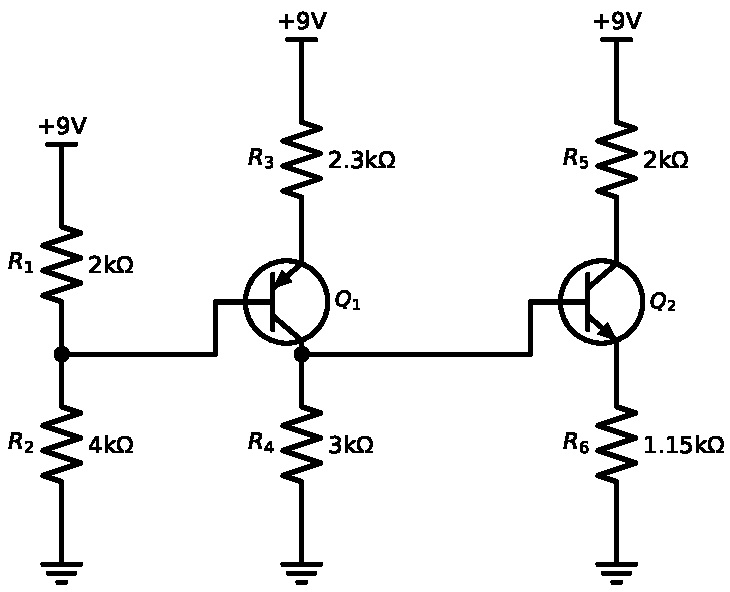
\includegraphics[width=0.9\linewidth,height=6cm,keepaspectratio]{p10_circuit}\end{center}
\solstep{1}{Assumptions}Assume every transistor is in the active region and that every base current is negligible ($I_B\approx0$, tool T1): then $|V_{BE}| = 0.7$\,V, $I_C\approx I_E$, and no current flows into any base, so a base network behaves like a plain resistor divider.
\solstep{2}{Walk through the circuit}\begin{enumerate}[leftmargin=*,itemsep=3pt]
\item No current flows into the base ($I_B$ is negligible), so $V_{B1}$ is set by the divider $R_{1}$--$R_{2}$ between $9$ and $0$ (Lecture-1 tool):\[V_{B1} = 0 + (9 - (0))\frac{4\,\mathrm{k}}{2\,\mathrm{k} + 4\,\mathrm{k}} = 6\,\mathrm{V}\]
\item $Q_{1}$ is pnp and assumed active: $V_{BE} = -0.7$\,V, so $V_{E1} = V_{B1} + 0.7 = 6.7\,\mathrm{V}$.
\item KCL at the emitter of $Q_{1}$ (base current neglected): \[I_{E1} = \frac{9 - V_{E1}}{R_{3}} = 1\,\mathrm{m}\mathrm{A}, \qquad I_{C1} \approx I_{E1}\]
\item The current $I_{C1} = 1\,\mathrm{m}\mathrm{A}$ flows from $V_{C1}$ through $R_{4}$: $V_{C1} = 0 + R_{4}\,(I_{C1}) = 0 + 3\,\mathrm{k}\times1\,\mathrm{m}\mathrm{A} = 3\,\mathrm{V}$.
\item $Q_{2}$ is npn and assumed active: $V_{BE} = 0.7$\,V, so $V_{E2} = V_{C1} - 0.7 = 2.3\,\mathrm{V}$.
\item KCL at the emitter of $Q_{2}$ (base current neglected): \[I_{E2} = \frac{V_{E2} - 0}{R_{6}} = 2\,\mathrm{m}\mathrm{A}, \qquad I_{C2} \approx I_{E2}\]
\item $Q_{2}$ draws $I_{C2} = 2\,\mathrm{m}\mathrm{A}$ from $V_{C2}$ through $R_{5}$: $V_{C2} = 9 - R_{5}\,(I_{C2}) = 9 - 2\,\mathrm{k}\times2\,\mathrm{m}\mathrm{A} = 5\,\mathrm{V}$.
\end{enumerate}

\solstep{3}{Verify the assumptions}\begin{itemize}[leftmargin=*,itemsep=2pt]
\item $I_{B1} = \frac{I_{C1}}{\beta} = 10\,\mu \mathrm{A}$ $\ll$ the $1.5\,\mathrm{m}\mathrm{A}$ flowing in the base network \checkmark
\item $I_{B2} = \frac{I_{C2}}{\beta} = 20\,\mu \mathrm{A}$ $\ll$ the $1\,\mathrm{m}\mathrm{A}$ flowing in the base network \checkmark
\item $V_{EC1} = V_{E1} - V_{C1} = 6.7 - (3) = 3.7\,\mathrm{V}$ $\ge 0.2$\,V $\Rightarrow$ $Q_{1}$ is active \checkmark
\item $V_{CE2} = V_{C2} - V_{E2} = 5 - (2.3) = 2.7\,\mathrm{V}$ $\ge 0.2$\,V $\Rightarrow$ $Q_{2}$ is active \checkmark
\end{itemize}

\solstep{4}{How good was $I_B\approx 0$?}If we keep the base currents ($I_C=\beta I_B$ with $\beta=100$) and solve the circuit exactly, the currents change only a little:\begin{center}\renewcommand{\arraystretch}{1.35}
\begin{tabular}{cccc}
\toprule
transistor & $I_C$ (with $I_B\approx0$) & $I_C$ (exact) & difference \\
\midrule
$Q_{1}$ & $1\,\mathrm{m}\mathrm{A}$ & $984\,\mu \mathrm{A}$ & $1.6\%$ \\
$Q_{2}$ & $2\,\mathrm{m}\mathrm{A}$ & $1.89\,\mathrm{m}\mathrm{A}$ & $5.8\%$ \\
\bottomrule
\end{tabular}\end{center}

\begin{ansbox}
$I_{C1} = 1\,\mathrm{m}\mathrm{A}$,\quad $I_{C2} = 2\,\mathrm{m}\mathrm{A}$\\[2pt] all transistors active, all base currents negligible.
\end{ansbox}

\newpage
\subsection*{Solution 4A.11 \hfill Medium}
\begin{center}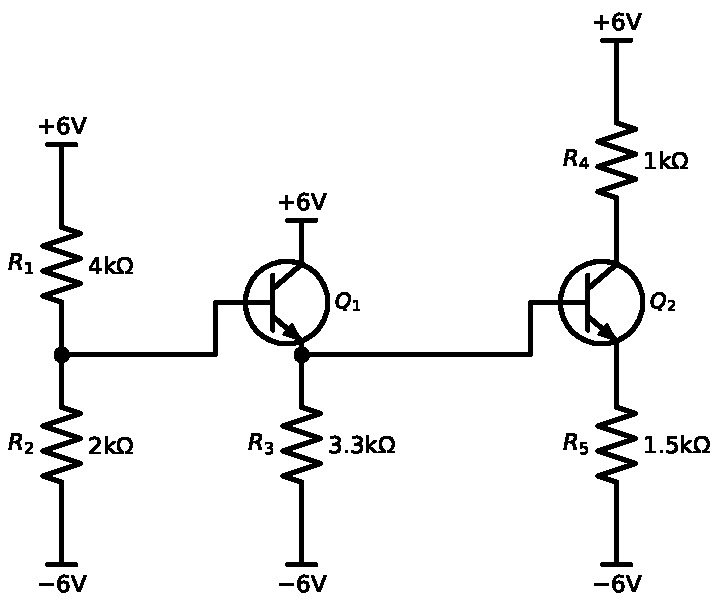
\includegraphics[width=0.9\linewidth,height=6cm,keepaspectratio]{p11_circuit}\end{center}
\solstep{1}{Assumptions}Assume every transistor is in the active region and that every base current is negligible ($I_B\approx0$, tool T1): then $|V_{BE}| = 0.7$\,V, $I_C\approx I_E$, and no current flows into any base, so a base network behaves like a plain resistor divider.
\solstep{2}{Walk through the circuit}\begin{enumerate}[leftmargin=*,itemsep=3pt]
\item No current flows into the base ($I_B$ is negligible), so $V_{B1}$ is set by the divider $R_{1}$--$R_{2}$ between $6$ and $(-6)$ (Lecture-1 tool):\[V_{B1} = -6 + (6 - (-6))\frac{2\,\mathrm{k}}{4\,\mathrm{k} + 2\,\mathrm{k}} = -2\,\mathrm{V}\]
\item $Q_{1}$ is npn and assumed active: $V_{BE} = 0.7$\,V, so $V_{E1} = V_{B1} - 0.7 = -2.7\,\mathrm{V}$.
\item $Q_{2}$ is npn and assumed active: $V_{BE} = 0.7$\,V, so $V_{E2} = V_{E1} - 0.7 = -3.4\,\mathrm{V}$.
\item KCL at the emitter of $Q_{1}$ (base current neglected): \[I_{E1} = \frac{V_{E1} - (-6)}{R_{3}} = 1\,\mathrm{m}\mathrm{A}, \qquad I_{C1} \approx I_{E1}\]
\item KCL at the emitter of $Q_{2}$ (base current neglected): \[I_{E2} = \frac{V_{E2} - (-6)}{R_{5}} = 1.73\,\mathrm{m}\mathrm{A}, \qquad I_{C2} \approx I_{E2}\]
\item $Q_{2}$ draws $I_{C2} = 1.73\,\mathrm{m}\mathrm{A}$ from $V_{C2}$ through $R_{4}$: $V_{C2} = 6 - R_{4}\,(I_{C2}) = 6 - 1\,\mathrm{k}\times1.73\,\mathrm{m}\mathrm{A} = 4.27\,\mathrm{V}$.
\end{enumerate}

\solstep{3}{Verify the assumptions}\begin{itemize}[leftmargin=*,itemsep=2pt]
\item $I_{B1} = \frac{I_{C1}}{\beta} = 10\,\mu \mathrm{A}$ $\ll$ the $2\,\mathrm{m}\mathrm{A}$ flowing in the base network \checkmark
\item $I_{B2} = \frac{I_{C2}}{\beta} = 17.3\,\mu \mathrm{A}$ $\ll$ the $1\,\mathrm{m}\mathrm{A}$ flowing in the base network \checkmark
\item $V_{CE1} = 6 - V_{E1} = 6 - (-2.7) = 8.7\,\mathrm{V}$ $\ge 0.2$\,V $\Rightarrow$ $Q_{1}$ is active \checkmark
\item $V_{CE2} = V_{C2} - V_{E2} = 4.267 - (-3.4) = 7.67\,\mathrm{V}$ $\ge 0.2$\,V $\Rightarrow$ $Q_{2}$ is active \checkmark
\end{itemize}

\solstep{4}{How good was $I_B\approx 0$?}If we keep the base currents ($I_C=\beta I_B$ with $\beta=100$) and solve the circuit exactly, the currents change only a little:\begin{center}\renewcommand{\arraystretch}{1.35}
\begin{tabular}{cccc}
\toprule
transistor & $I_C$ (with $I_B\approx0$) & $I_C$ (exact) & difference \\
\midrule
$Q_{1}$ & $1\,\mathrm{m}\mathrm{A}$ & $1\,\mathrm{m}\mathrm{A}$ & $-0.3\%$ \\
$Q_{2}$ & $1.73\,\mathrm{m}\mathrm{A}$ & $1.71\,\mathrm{m}\mathrm{A}$ & $1.5\%$ \\
\bottomrule
\end{tabular}\end{center}

\begin{ansbox}
$I_{C1} = 1\,\mathrm{m}\mathrm{A}$,\quad $I_{C2} = 1.73\,\mathrm{m}\mathrm{A}$\\[2pt] all transistors active, all base currents negligible.
\end{ansbox}

\newpage
\subsection*{Solution 4A.12 \hfill Medium}
\begin{center}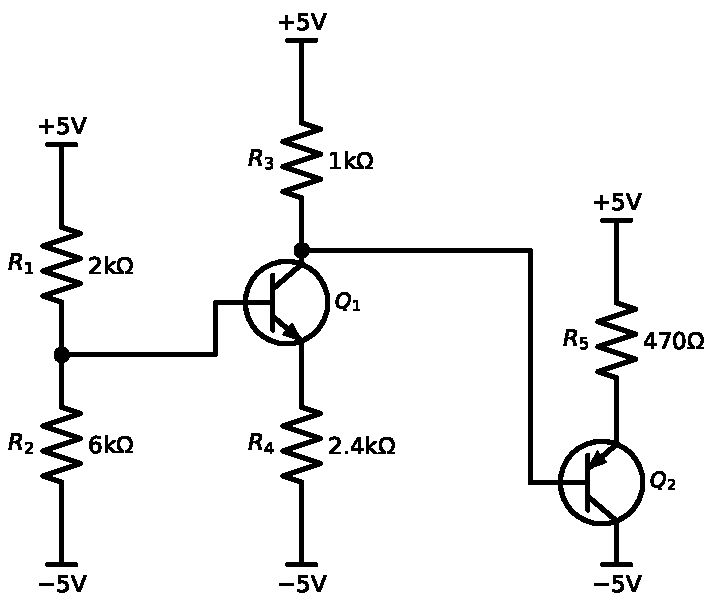
\includegraphics[width=0.9\linewidth,height=6cm,keepaspectratio]{p12_circuit}\end{center}
\solstep{1}{Assumptions}Assume every transistor is in the active region and that every base current is negligible ($I_B\approx0$, tool T1): then $|V_{BE}| = 0.7$\,V, $I_C\approx I_E$, and no current flows into any base, so a base network behaves like a plain resistor divider.
\solstep{2}{Walk through the circuit}\begin{enumerate}[leftmargin=*,itemsep=3pt]
\item No current flows into the base ($I_B$ is negligible), so $V_{B1}$ is set by the divider $R_{1}$--$R_{2}$ between $5$ and $(-5)$ (Lecture-1 tool):\[V_{B1} = -5 + (5 - (-5))\frac{6\,\mathrm{k}}{2\,\mathrm{k} + 6\,\mathrm{k}} = 2.5\,\mathrm{V}\]
\item $Q_{1}$ is npn and assumed active: $V_{BE} = 0.7$\,V, so $V_{E1} = V_{B1} - 0.7 = 1.8\,\mathrm{V}$.
\item KCL at the emitter of $Q_{1}$ (base current neglected): \[I_{E1} = \frac{V_{E1} - (-5)}{R_{4}} = 2.83\,\mathrm{m}\mathrm{A}, \qquad I_{C1} \approx I_{E1}\]
\item $Q_{1}$ draws $I_{C1} = 2.83\,\mathrm{m}\mathrm{A}$ from $V_{C1}$ through $R_{3}$: $V_{C1} = 5 - R_{3}\,(I_{C1}) = 5 - 1\,\mathrm{k}\times2.83\,\mathrm{m}\mathrm{A} = 2.17\,\mathrm{V}$.
\item $Q_{2}$ is pnp and assumed active: $V_{BE} = -0.7$\,V, so $V_{E2} = V_{C1} + 0.7 = 2.87\,\mathrm{V}$.
\item KCL at the emitter of $Q_{2}$ (base current neglected): \[I_{E2} = \frac{5 - V_{E2}}{R_{5}} = 4.54\,\mathrm{m}\mathrm{A}, \qquad I_{C2} \approx I_{E2}\]
\end{enumerate}

\solstep{3}{Verify the assumptions}\begin{itemize}[leftmargin=*,itemsep=2pt]
\item $I_{B1} = \frac{I_{C1}}{\beta} = 28.3\,\mu \mathrm{A}$ $\ll$ the $1.25\,\mathrm{m}\mathrm{A}$ flowing in the base network \checkmark
\item $I_{B2} = \frac{I_{C2}}{\beta} = 45.4\,\mu \mathrm{A}$ $\ll$ the $2.83\,\mathrm{m}\mathrm{A}$ flowing in the base network \checkmark
\item $V_{CE1} = V_{C1} - V_{E1} = 2.167 - (1.8) = 0.367\,\mathrm{V}$ $\ge 0.2$\,V $\Rightarrow$ $Q_{1}$ is active \checkmark
\item $V_{EC2} = V_{E2} - (-5) = 2.867 - (-5) = 7.87\,\mathrm{V}$ $\ge 0.2$\,V $\Rightarrow$ $Q_{2}$ is active \checkmark
\end{itemize}

\solstep{4}{How good was $I_B\approx 0$?}If we keep the base currents ($I_C=\beta I_B$ with $\beta=100$) and solve the circuit exactly, the currents change only a little:\begin{center}\renewcommand{\arraystretch}{1.35}
\begin{tabular}{cccc}
\toprule
transistor & $I_C$ (with $I_B\approx0$) & $I_C$ (exact) & difference \\
\midrule
$Q_{1}$ & $2.83\,\mathrm{m}\mathrm{A}$ & $2.79\,\mathrm{m}\mathrm{A}$ & $1.6\%$ \\
$Q_{2}$ & $4.54\,\mathrm{m}\mathrm{A}$ & $4.31\,\mathrm{m}\mathrm{A}$ & $5.4\%$ \\
\bottomrule
\end{tabular}\end{center}

\begin{ansbox}
$I_{C1} = 2.83\,\mathrm{m}\mathrm{A}$,\quad $I_{C2} = 4.54\,\mathrm{m}\mathrm{A}$\\[2pt] all transistors active, all base currents negligible.
\end{ansbox}

\newpage
\subsection*{Solution 4A.13 \hfill Hard}
\begin{center}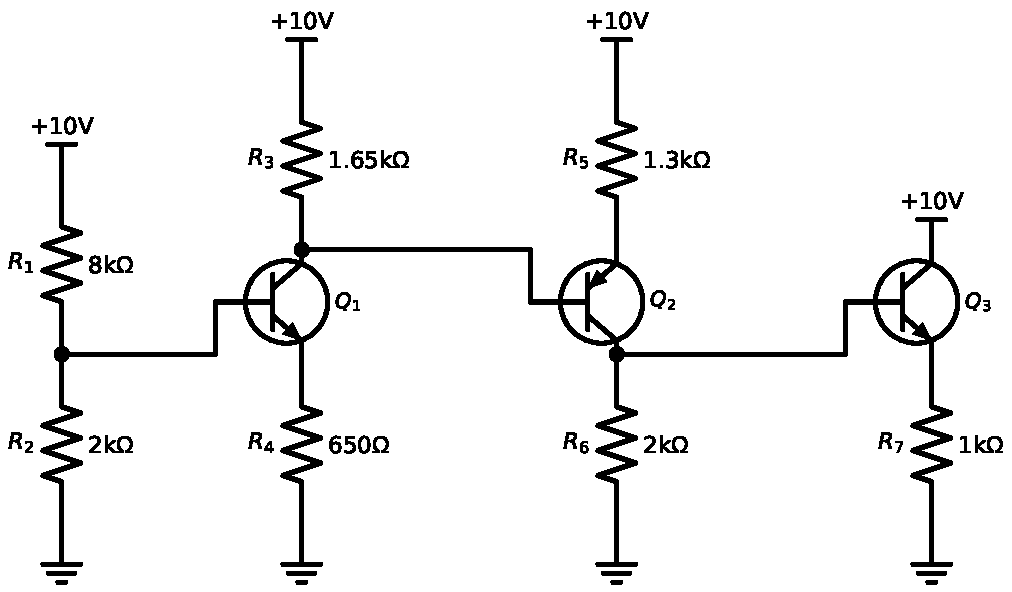
\includegraphics[width=0.9\linewidth,height=6cm,keepaspectratio]{p13_circuit}\end{center}
\solstep{1}{Assumptions}Assume every transistor is in the active region and that every base current is negligible ($I_B\approx0$, tool T1): then $|V_{BE}| = 0.7$\,V, $I_C\approx I_E$, and no current flows into any base, so a base network behaves like a plain resistor divider.
\solstep{2}{Walk through the circuit}\begin{enumerate}[leftmargin=*,itemsep=3pt]
\item No current flows into the base ($I_B$ is negligible), so $V_{B1}$ is set by the divider $R_{1}$--$R_{2}$ between $10$ and $0$ (Lecture-1 tool):\[V_{B1} = 0 + (10 - (0))\frac{2\,\mathrm{k}}{8\,\mathrm{k} + 2\,\mathrm{k}} = 2\,\mathrm{V}\]
\item $Q_{1}$ is npn and assumed active: $V_{BE} = 0.7$\,V, so $V_{E1} = V_{B1} - 0.7 = 1.3\,\mathrm{V}$.
\item KCL at the emitter of $Q_{1}$ (base current neglected): \[I_{E1} = \frac{V_{E1} - 0}{R_{4}} = 2\,\mathrm{m}\mathrm{A}, \qquad I_{C1} \approx I_{E1}\]
\item $Q_{1}$ draws $I_{C1} = 2\,\mathrm{m}\mathrm{A}$ from $V_{C1}$ through $R_{3}$: $V_{C1} = 10 - R_{3}\,(I_{C1}) = 10 - 1.65\,\mathrm{k}\times2\,\mathrm{m}\mathrm{A} = 6.7\,\mathrm{V}$.
\item $Q_{2}$ is pnp and assumed active: $V_{BE} = -0.7$\,V, so $V_{E2} = V_{C1} + 0.7 = 7.4\,\mathrm{V}$.
\item KCL at the emitter of $Q_{2}$ (base current neglected): \[I_{E2} = \frac{10 - V_{E2}}{R_{5}} = 2\,\mathrm{m}\mathrm{A}, \qquad I_{C2} \approx I_{E2}\]
\item The current $I_{C2} = 2\,\mathrm{m}\mathrm{A}$ flows from $V_{C2}$ through $R_{6}$: $V_{C2} = 0 + R_{6}\,(I_{C2}) = 0 + 2\,\mathrm{k}\times2\,\mathrm{m}\mathrm{A} = 4\,\mathrm{V}$.
\item $Q_{3}$ is npn and assumed active: $V_{BE} = 0.7$\,V, so $V_{E3} = V_{C2} - 0.7 = 3.3\,\mathrm{V}$.
\item KCL at the emitter of $Q_{3}$ (base current neglected): \[I_{E3} = \frac{V_{E3} - 0}{R_{7}} = 3.3\,\mathrm{m}\mathrm{A}, \qquad I_{C3} \approx I_{E3}\]
\end{enumerate}

\solstep{3}{Verify the assumptions}\begin{itemize}[leftmargin=*,itemsep=2pt]
\item $I_{B1} = \frac{I_{C1}}{\beta} = 20\,\mu \mathrm{A}$ $\ll$ the $1\,\mathrm{m}\mathrm{A}$ flowing in the base network \checkmark
\item $I_{B2} = \frac{I_{C2}}{\beta} = 20\,\mu \mathrm{A}$ $\ll$ the $2\,\mathrm{m}\mathrm{A}$ flowing in the base network \checkmark
\item $I_{B3} = \frac{I_{C3}}{\beta} = 33\,\mu \mathrm{A}$ $\ll$ the $2\,\mathrm{m}\mathrm{A}$ flowing in the base network \checkmark
\item $V_{CE1} = V_{C1} - V_{E1} = 6.7 - (1.3) = 5.4\,\mathrm{V}$ $\ge 0.2$\,V $\Rightarrow$ $Q_{1}$ is active \checkmark
\item $V_{EC2} = V_{E2} - V_{C2} = 7.4 - (4) = 3.4\,\mathrm{V}$ $\ge 0.2$\,V $\Rightarrow$ $Q_{2}$ is active \checkmark
\item $V_{CE3} = 10 - V_{E3} = 10 - (3.3) = 6.7\,\mathrm{V}$ $\ge 0.2$\,V $\Rightarrow$ $Q_{3}$ is active \checkmark
\end{itemize}

\solstep{4}{How good was $I_B\approx 0$?}If we keep the base currents ($I_C=\beta I_B$ with $\beta=100$) and solve the circuit exactly, the currents change only a little:\begin{center}\renewcommand{\arraystretch}{1.35}
\begin{tabular}{cccc}
\toprule
transistor & $I_C$ (with $I_B\approx0$) & $I_C$ (exact) & difference \\
\midrule
$Q_{1}$ & $2\,\mathrm{m}\mathrm{A}$ & $1.93\,\mathrm{m}\mathrm{A}$ & $3.5\%$ \\
$Q_{2}$ & $2\,\mathrm{m}\mathrm{A}$ & $1.87\,\mathrm{m}\mathrm{A}$ & $6.8\%$ \\
$Q_{3}$ & $3.3\,\mathrm{m}\mathrm{A}$ & $2.96\,\mathrm{m}\mathrm{A}$ & $12\%$ \\
\bottomrule
\end{tabular}\end{center}
 The differences grow along the chain: every base current slightly shifts the collector voltage that biases the next transistor, and $\alpha = \beta/(\beta+1)$ makes each $I_C$ about 1\,\% smaller than its $I_E$. A shift is amplified when the next stage has only a small voltage across its emitter resistor. Hand analysis with $I_B\approx0$ is still the standard first pass.
\begin{ansbox}
$I_{C1} = 2\,\mathrm{m}\mathrm{A}$,\quad $I_{C2} = 2\,\mathrm{m}\mathrm{A}$,\quad $I_{C3} = 3.3\,\mathrm{m}\mathrm{A}$\\[2pt] all transistors active, all base currents negligible.
\end{ansbox}

\newpage
\subsection*{Solution 4A.14 \hfill Hard}
\begin{center}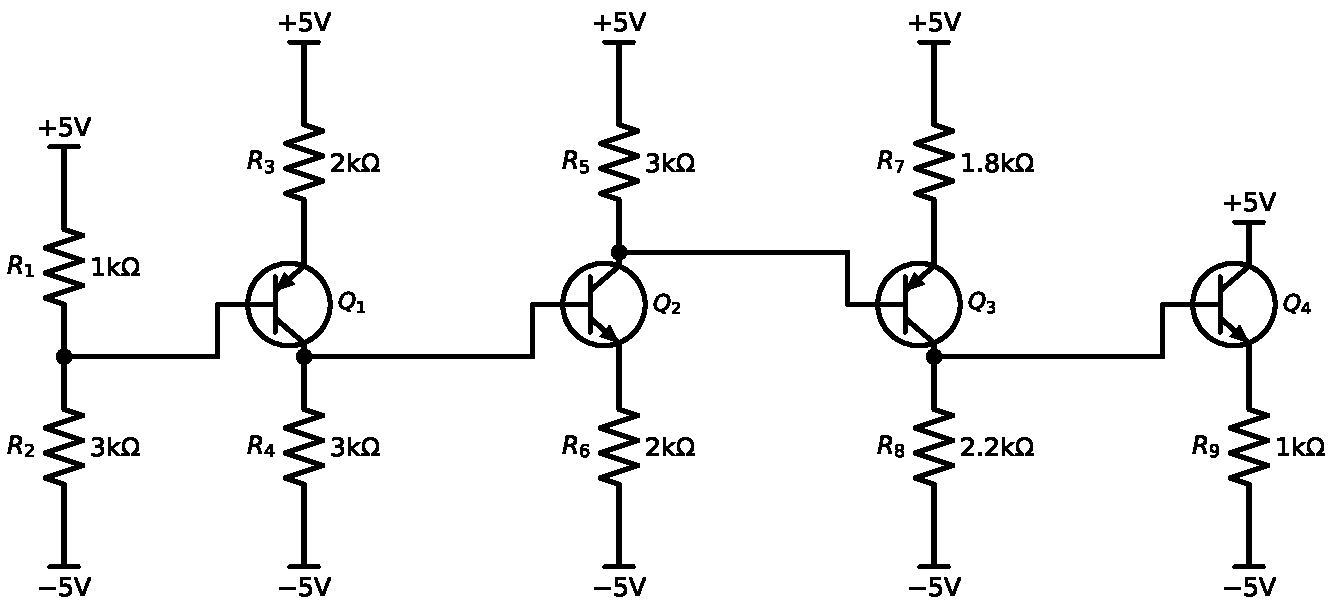
\includegraphics[width=0.9\linewidth,height=6cm,keepaspectratio]{p14_circuit}\end{center}
\solstep{1}{Assumptions}Assume every transistor is in the active region and that every base current is negligible ($I_B\approx0$, tool T1): then $|V_{BE}| = 0.7$\,V, $I_C\approx I_E$, and no current flows into any base, so a base network behaves like a plain resistor divider.
\solstep{2}{Walk through the circuit}\begin{enumerate}[leftmargin=*,itemsep=3pt]
\item No current flows into the base ($I_B$ is negligible), so $V_{B1}$ is set by the divider $R_{1}$--$R_{2}$ between $5$ and $(-5)$ (Lecture-1 tool):\[V_{B1} = -5 + (5 - (-5))\frac{3\,\mathrm{k}}{1\,\mathrm{k} + 3\,\mathrm{k}} = 2.5\,\mathrm{V}\]
\item $Q_{1}$ is pnp and assumed active: $V_{BE} = -0.7$\,V, so $V_{E1} = V_{B1} + 0.7 = 3.2\,\mathrm{V}$.
\item KCL at the emitter of $Q_{1}$ (base current neglected): \[I_{E1} = \frac{5 - V_{E1}}{R_{3}} = 900\,\mu \mathrm{A}, \qquad I_{C1} \approx I_{E1}\]
\item The current $I_{C1} = 900\,\mu \mathrm{A}$ flows from $V_{C1}$ through $R_{4}$: $V_{C1} = (-5) + R_{4}\,(I_{C1}) = -5 + 3\,\mathrm{k}\times900\,\mu \mathrm{A} = -2.3\,\mathrm{V}$.
\item $Q_{2}$ is npn and assumed active: $V_{BE} = 0.7$\,V, so $V_{E2} = V_{C1} - 0.7 = -3\,\mathrm{V}$.
\item KCL at the emitter of $Q_{2}$ (base current neglected): \[I_{E2} = \frac{V_{E2} - (-5)}{R_{6}} = 1\,\mathrm{m}\mathrm{A}, \qquad I_{C2} \approx I_{E2}\]
\item $Q_{2}$ draws $I_{C2} = 1\,\mathrm{m}\mathrm{A}$ from $V_{C2}$ through $R_{5}$: $V_{C2} = 5 - R_{5}\,(I_{C2}) = 5 - 3\,\mathrm{k}\times1\,\mathrm{m}\mathrm{A} = 2\,\mathrm{V}$.
\item $Q_{3}$ is pnp and assumed active: $V_{BE} = -0.7$\,V, so $V_{E3} = V_{C2} + 0.7 = 2.7\,\mathrm{V}$.
\item KCL at the emitter of $Q_{3}$ (base current neglected): \[I_{E3} = \frac{5 - V_{E3}}{R_{7}} = 1.28\,\mathrm{m}\mathrm{A}, \qquad I_{C3} \approx I_{E3}\]
\item The current $I_{C3} = 1.28\,\mathrm{m}\mathrm{A}$ flows from $V_{C3}$ through $R_{8}$: $V_{C3} = (-5) + R_{8}\,(I_{C3}) = -5 + 2.2\,\mathrm{k}\times1.28\,\mathrm{m}\mathrm{A} = -2.19\,\mathrm{V}$.
\item $Q_{4}$ is npn and assumed active: $V_{BE} = 0.7$\,V, so $V_{E4} = V_{C3} - 0.7 = -2.89\,\mathrm{V}$.
\item KCL at the emitter of $Q_{4}$ (base current neglected): \[I_{E4} = \frac{V_{E4} - (-5)}{R_{9}} = 2.11\,\mathrm{m}\mathrm{A}, \qquad I_{C4} \approx I_{E4}\]
\end{enumerate}

\solstep{3}{Verify the assumptions}\begin{itemize}[leftmargin=*,itemsep=2pt]
\item $I_{B1} = \frac{I_{C1}}{\beta} = 9\,\mu \mathrm{A}$ $\ll$ the $2.5\,\mathrm{m}\mathrm{A}$ flowing in the base network \checkmark
\item $I_{B2} = \frac{I_{C2}}{\beta} = 10\,\mu \mathrm{A}$ $\ll$ the $900\,\mu \mathrm{A}$ flowing in the base network \checkmark
\item $I_{B3} = \frac{I_{C3}}{\beta} = 12.8\,\mu \mathrm{A}$ $\ll$ the $1\,\mathrm{m}\mathrm{A}$ flowing in the base network \checkmark
\item $I_{B4} = \frac{I_{C4}}{\beta} = 21.1\,\mu \mathrm{A}$ $\ll$ the $1.28\,\mathrm{m}\mathrm{A}$ flowing in the base network \checkmark
\item $V_{EC1} = V_{E1} - V_{C1} = 3.2 - (-2.3) = 5.5\,\mathrm{V}$ $\ge 0.2$\,V $\Rightarrow$ $Q_{1}$ is active \checkmark
\item $V_{CE2} = V_{C2} - V_{E2} = 2 - (-3) = 5\,\mathrm{V}$ $\ge 0.2$\,V $\Rightarrow$ $Q_{2}$ is active \checkmark
\item $V_{EC3} = V_{E3} - V_{C3} = 2.7 - (-2.189) = 4.89\,\mathrm{V}$ $\ge 0.2$\,V $\Rightarrow$ $Q_{3}$ is active \checkmark
\item $V_{CE4} = 5 - V_{E4} = 5 - (-2.889) = 7.89\,\mathrm{V}$ $\ge 0.2$\,V $\Rightarrow$ $Q_{4}$ is active \checkmark
\end{itemize}

\solstep{4}{How good was $I_B\approx 0$?}If we keep the base currents ($I_C=\beta I_B$ with $\beta=100$) and solve the circuit exactly, the currents change only a little:\begin{center}\renewcommand{\arraystretch}{1.35}
\begin{tabular}{cccc}
\toprule
transistor & $I_C$ (with $I_B\approx0$) & $I_C$ (exact) & difference \\
\midrule
$Q_{1}$ & $900\,\mu \mathrm{A}$ & $888\,\mu \mathrm{A}$ & $1.4\%$ \\
$Q_{2}$ & $1\,\mathrm{m}\mathrm{A}$ & $958\,\mu \mathrm{A}$ & $4.4\%$ \\
$Q_{3}$ & $1.28\,\mathrm{m}\mathrm{A}$ & $1.18\,\mathrm{m}\mathrm{A}$ & $8.7\%$ \\
$Q_{4}$ & $2.11\,\mathrm{m}\mathrm{A}$ & $1.83\,\mathrm{m}\mathrm{A}$ & $15\%$ \\
\bottomrule
\end{tabular}\end{center}
 The differences grow along the chain: every base current slightly shifts the collector voltage that biases the next transistor, and $\alpha = \beta/(\beta+1)$ makes each $I_C$ about 1\,\% smaller than its $I_E$. A shift is amplified when the next stage has only a small voltage across its emitter resistor. Hand analysis with $I_B\approx0$ is still the standard first pass.
\begin{ansbox}
$I_{C1} = 900\,\mu \mathrm{A}$,\quad $I_{C2} = 1\,\mathrm{m}\mathrm{A}$,\quad $I_{C3} = 1.28\,\mathrm{m}\mathrm{A}$,\quad $I_{C4} = 2.11\,\mathrm{m}\mathrm{A}$\\[2pt] all transistors active, all base currents negligible.
\end{ansbox}

\newpage
\subsection*{Solution 4A.15 \hfill Hard}
\begin{center}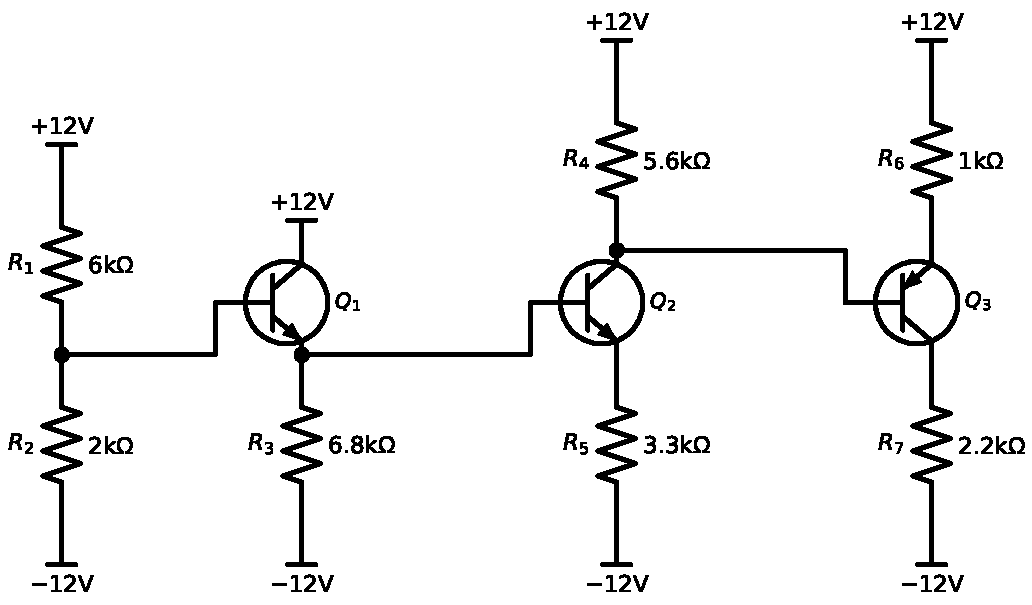
\includegraphics[width=0.9\linewidth,height=6cm,keepaspectratio]{p15_circuit}\end{center}
\solstep{1}{Assumptions}Assume every transistor is in the active region and that every base current is negligible ($I_B\approx0$, tool T1): then $|V_{BE}| = 0.7$\,V, $I_C\approx I_E$, and no current flows into any base, so a base network behaves like a plain resistor divider.
\solstep{2}{Walk through the circuit}\begin{enumerate}[leftmargin=*,itemsep=3pt]
\item No current flows into the base ($I_B$ is negligible), so $V_{B1}$ is set by the divider $R_{1}$--$R_{2}$ between $12$ and $(-12)$ (Lecture-1 tool):\[V_{B1} = -12 + (12 - (-12))\frac{2\,\mathrm{k}}{6\,\mathrm{k} + 2\,\mathrm{k}} = -6\,\mathrm{V}\]
\item $Q_{1}$ is npn and assumed active: $V_{BE} = 0.7$\,V, so $V_{E1} = V_{B1} - 0.7 = -6.7\,\mathrm{V}$.
\item $Q_{2}$ is npn and assumed active: $V_{BE} = 0.7$\,V, so $V_{E2} = V_{E1} - 0.7 = -7.4\,\mathrm{V}$.
\item KCL at the emitter of $Q_{1}$ (base current neglected): \[I_{E1} = \frac{V_{E1} - (-12)}{R_{3}} = 779\,\mu \mathrm{A}, \qquad I_{C1} \approx I_{E1}\]
\item KCL at the emitter of $Q_{2}$ (base current neglected): \[I_{E2} = \frac{V_{E2} - (-12)}{R_{5}} = 1.39\,\mathrm{m}\mathrm{A}, \qquad I_{C2} \approx I_{E2}\]
\item $Q_{2}$ draws $I_{C2} = 1.39\,\mathrm{m}\mathrm{A}$ from $V_{C2}$ through $R_{4}$: $V_{C2} = 12 - R_{4}\,(I_{C2}) = 12 - 5.6\,\mathrm{k}\times1.39\,\mathrm{m}\mathrm{A} = 4.19\,\mathrm{V}$.
\item $Q_{3}$ is pnp and assumed active: $V_{BE} = -0.7$\,V, so $V_{E3} = V_{C2} + 0.7 = 4.89\,\mathrm{V}$.
\item KCL at the emitter of $Q_{3}$ (base current neglected): \[I_{E3} = \frac{12 - V_{E3}}{R_{6}} = 7.11\,\mathrm{m}\mathrm{A}, \qquad I_{C3} \approx I_{E3}\]
\item The current $I_{C3} = 7.11\,\mathrm{m}\mathrm{A}$ flows from $V_{C3}$ through $R_{7}$: $V_{C3} = (-12) + R_{7}\,(I_{C3}) = -12 + 2.2\,\mathrm{k}\times7.11\,\mathrm{m}\mathrm{A} = 3.63\,\mathrm{V}$.
\end{enumerate}

\solstep{3}{Verify the assumptions}\begin{itemize}[leftmargin=*,itemsep=2pt]
\item $I_{B1} = \frac{I_{C1}}{\beta} = 7.79\,\mu \mathrm{A}$ $\ll$ the $3\,\mathrm{m}\mathrm{A}$ flowing in the base network \checkmark
\item $I_{B2} = \frac{I_{C2}}{\beta} = 13.9\,\mu \mathrm{A}$ $\ll$ the $779\,\mu \mathrm{A}$ flowing in the base network \checkmark
\item $I_{B3} = \frac{I_{C3}}{\beta} = 71.1\,\mu \mathrm{A}$ $\ll$ the $1.39\,\mathrm{m}\mathrm{A}$ flowing in the base network \checkmark
\item $V_{CE1} = 12 - V_{E1} = 12 - (-6.7) = 18.7\,\mathrm{V}$ $\ge 0.2$\,V $\Rightarrow$ $Q_{1}$ is active \checkmark
\item $V_{CE2} = V_{C2} - V_{E2} = 4.194 - (-7.4) = 11.6\,\mathrm{V}$ $\ge 0.2$\,V $\Rightarrow$ $Q_{2}$ is active \checkmark
\item $V_{EC3} = V_{E3} - V_{C3} = 4.894 - (3.633) = 1.26\,\mathrm{V}$ $\ge 0.2$\,V $\Rightarrow$ $Q_{3}$ is active \checkmark
\end{itemize}

\solstep{4}{How good was $I_B\approx 0$?}If we keep the base currents ($I_C=\beta I_B$ with $\beta=100$) and solve the circuit exactly, the currents change only a little:\begin{center}\renewcommand{\arraystretch}{1.35}
\begin{tabular}{cccc}
\toprule
transistor & $I_C$ (with $I_B\approx0$) & $I_C$ (exact) & difference \\
\midrule
$Q_{1}$ & $779\,\mu \mathrm{A}$ & $784\,\mu \mathrm{A}$ & $-0.54\%$ \\
$Q_{2}$ & $1.39\,\mathrm{m}\mathrm{A}$ & $1.38\,\mathrm{m}\mathrm{A}$ & $1.3\%$ \\
$Q_{3}$ & $7.11\,\mathrm{m}\mathrm{A}$ & $6.58\,\mathrm{m}\mathrm{A}$ & $8.1\%$ \\
\bottomrule
\end{tabular}\end{center}
 The differences grow along the chain: every base current slightly shifts the collector voltage that biases the next transistor, and $\alpha = \beta/(\beta+1)$ makes each $I_C$ about 1\,\% smaller than its $I_E$. A shift is amplified when the next stage has only a small voltage across its emitter resistor. Hand analysis with $I_B\approx0$ is still the standard first pass.
\begin{ansbox}
$I_{C1} = 779\,\mu \mathrm{A}$,\quad $I_{C2} = 1.39\,\mathrm{m}\mathrm{A}$,\quad $I_{C3} = 7.11\,\mathrm{m}\mathrm{A}$\\[2pt] all transistors active, all base currents negligible.
\end{ansbox}

\newpage
\subsection*{Solution 4A.16 \hfill Hard}
\begin{center}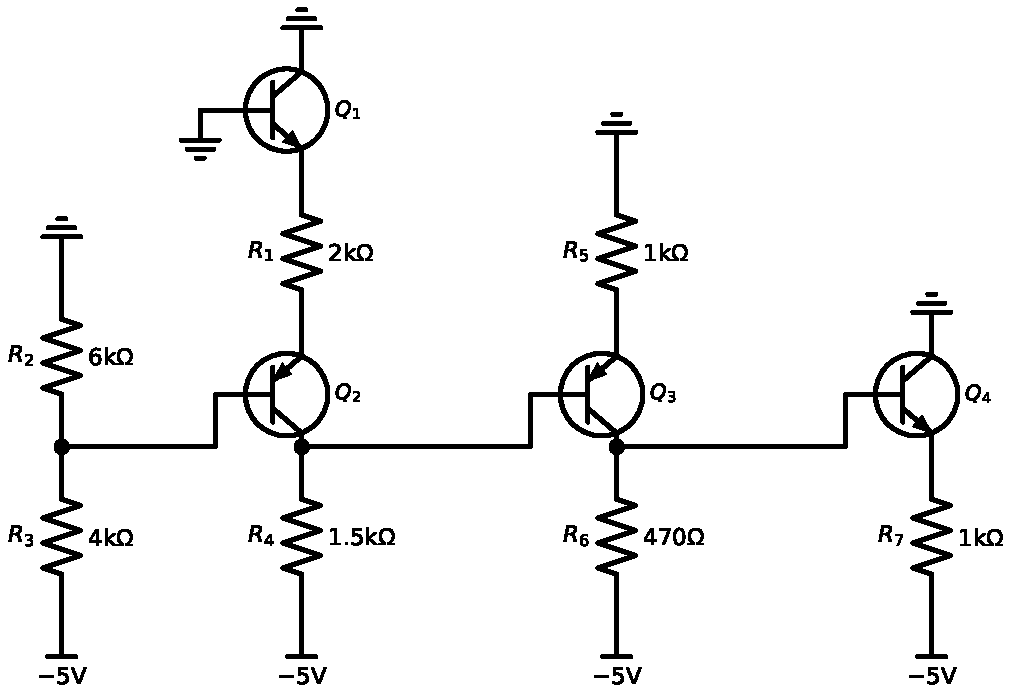
\includegraphics[width=0.9\linewidth,height=6cm,keepaspectratio]{p16_circuit}\end{center}
\solstep{1}{Assumptions}Assume every transistor is in the active region and that every base current is negligible ($I_B\approx0$, tool T1): then $|V_{BE}| = 0.7$\,V, $I_C\approx I_E$, and no current flows into any base, so a base network behaves like a plain resistor divider.
\solstep{2}{Walk through the circuit}\begin{enumerate}[leftmargin=*,itemsep=3pt]
\item $Q_{1}$ is npn and assumed active: $V_{BE} = 0.7$\,V, so $V_{E1} = 0 - 0.7 = -0.7\,\mathrm{V}$.
\item No current flows into the base ($I_B$ is negligible), so $V_{B2}$ is set by the divider $R_{2}$--$R_{3}$ between $0$ and $(-5)$ (Lecture-1 tool):\[V_{B2} = -5 + (0 - (-5))\frac{4\,\mathrm{k}}{6\,\mathrm{k} + 4\,\mathrm{k}} = -3\,\mathrm{V}\]
\item $Q_{2}$ is pnp and assumed active: $V_{BE} = -0.7$\,V, so $V_{E2} = V_{B2} + 0.7 = -2.3\,\mathrm{V}$.
\item KCL at the emitter of $Q_{1}$ (base current neglected): \[I_{E1} = \frac{V_{E1} - V_{E2}}{R_{1}} = 800\,\mu \mathrm{A}, \qquad I_{C1} \approx I_{E1}\]
\item KCL at the emitter of $Q_{2}$ (base current neglected): \[I_{E2} = \frac{V_{E1} - V_{E2}}{R_{1}} = 800\,\mu \mathrm{A}, \qquad I_{C2} \approx I_{E2}\]
\item The current $I_{C2} = 800\,\mu \mathrm{A}$ flows from $V_{C2}$ through $R_{4}$: $V_{C2} = (-5) + R_{4}\,(I_{C2}) = -5 + 1.5\,\mathrm{k}\times800\,\mu \mathrm{A} = -3.8\,\mathrm{V}$.
\item $Q_{3}$ is pnp and assumed active: $V_{BE} = -0.7$\,V, so $V_{E3} = V_{C2} + 0.7 = -3.1\,\mathrm{V}$.
\item KCL at the emitter of $Q_{3}$ (base current neglected): \[I_{E3} = \frac{0 - V_{E3}}{R_{5}} = 3.1\,\mathrm{m}\mathrm{A}, \qquad I_{C3} \approx I_{E3}\]
\item The current $I_{C3} = 3.1\,\mathrm{m}\mathrm{A}$ flows from $V_{C3}$ through $R_{6}$: $V_{C3} = (-5) + R_{6}\,(I_{C3}) = -5 + 470\times3.1\,\mathrm{m}\mathrm{A} = -3.54\,\mathrm{V}$.
\item $Q_{4}$ is npn and assumed active: $V_{BE} = 0.7$\,V, so $V_{E4} = V_{C3} - 0.7 = -4.24\,\mathrm{V}$.
\item KCL at the emitter of $Q_{4}$ (base current neglected): \[I_{E4} = \frac{V_{E4} - (-5)}{R_{7}} = 757\,\mu \mathrm{A}, \qquad I_{C4} \approx I_{E4}\]
\end{enumerate}

\solstep{3}{Verify the assumptions}\begin{itemize}[leftmargin=*,itemsep=2pt]
\item $I_{B1} = \frac{I_{C1}}{\beta} = 8\,\mu \mathrm{A}$ $\ll$ the $3.1\,\mathrm{m}\mathrm{A}$ flowing in the base network \checkmark
\item $I_{B2} = \frac{I_{C2}}{\beta} = 8\,\mu \mathrm{A}$ $\ll$ the $500\,\mu \mathrm{A}$ flowing in the base network \checkmark
\item $I_{B3} = \frac{I_{C3}}{\beta} = 31\,\mu \mathrm{A}$ $\ll$ the $800\,\mu \mathrm{A}$ flowing in the base network \checkmark
\item $I_{B4} = \frac{I_{C4}}{\beta} = 7.57\,\mu \mathrm{A}$ $\ll$ the $3.1\,\mathrm{m}\mathrm{A}$ flowing in the base network \checkmark
\item $V_{CE1} = 0 - V_{E1} = 0 - (-0.7) = 0.7\,\mathrm{V}$ $\ge 0.2$\,V $\Rightarrow$ $Q_{1}$ is active \checkmark
\item $V_{EC2} = V_{E2} - V_{C2} = -2.3 - (-3.8) = 1.5\,\mathrm{V}$ $\ge 0.2$\,V $\Rightarrow$ $Q_{2}$ is active \checkmark
\item $V_{EC3} = V_{E3} - V_{C3} = -3.1 - (-3.543) = 0.443\,\mathrm{V}$ $\ge 0.2$\,V $\Rightarrow$ $Q_{3}$ is active \checkmark
\item $V_{CE4} = 0 - V_{E4} = 0 - (-4.243) = 4.24\,\mathrm{V}$ $\ge 0.2$\,V $\Rightarrow$ $Q_{4}$ is active \checkmark
\end{itemize}

\solstep{4}{How good was $I_B\approx 0$?}If we keep the base currents ($I_C=\beta I_B$ with $\beta=100$) and solve the circuit exactly, the currents change only a little:\begin{center}\renewcommand{\arraystretch}{1.35}
\begin{tabular}{cccc}
\toprule
transistor & $I_C$ (with $I_B\approx0$) & $I_C$ (exact) & difference \\
\midrule
$Q_{1}$ & $800\,\mu \mathrm{A}$ & $783\,\mu \mathrm{A}$ & $2.2\%$ \\
$Q_{2}$ & $800\,\mu \mathrm{A}$ & $783\,\mu \mathrm{A}$ & $2.2\%$ \\
$Q_{3}$ & $3.1\,\mathrm{m}\mathrm{A}$ & $3.05\,\mathrm{m}\mathrm{A}$ & $1.7\%$ \\
$Q_{4}$ & $757\,\mu \mathrm{A}$ & $723\,\mu \mathrm{A}$ & $4.7\%$ \\
\bottomrule
\end{tabular}\end{center}

\begin{ansbox}
$I_{C1} = 800\,\mu \mathrm{A}$,\quad $I_{C2} = 800\,\mu \mathrm{A}$,\quad $I_{C3} = 3.1\,\mathrm{m}\mathrm{A}$,\quad $I_{C4} = 757\,\mu \mathrm{A}$\\[2pt] all transistors active, all base currents negligible.
\end{ansbox}

\newpage
\subsection*{Solution 4A.17 \hfill Hard}
\begin{center}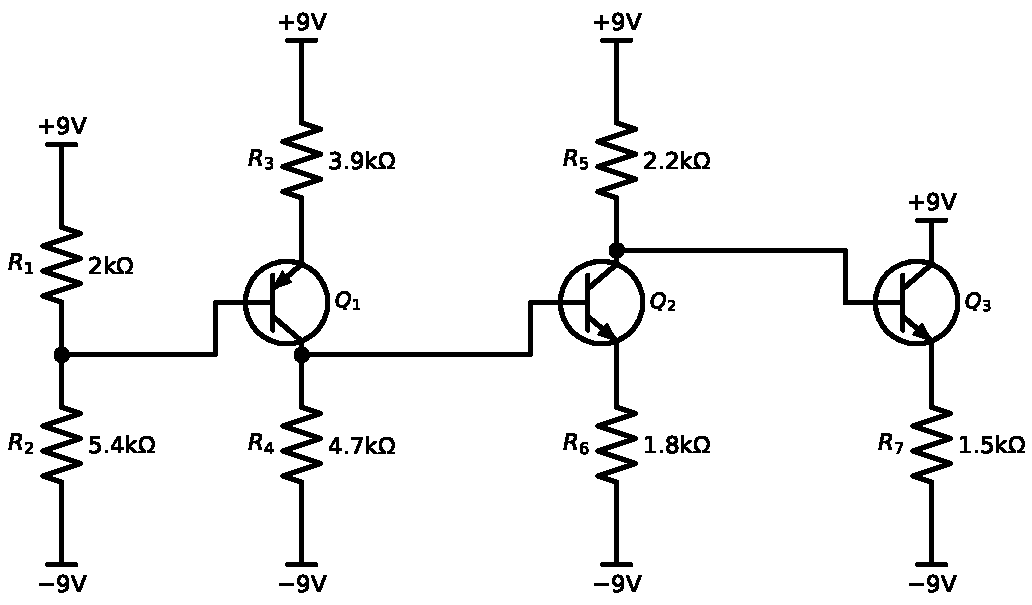
\includegraphics[width=0.9\linewidth,height=6cm,keepaspectratio]{p17_circuit}\end{center}
\solstep{1}{Assumptions}Assume every transistor is in the active region and that every base current is negligible ($I_B\approx0$, tool T1): then $|V_{BE}| = 0.7$\,V, $I_C\approx I_E$, and no current flows into any base, so a base network behaves like a plain resistor divider.
\solstep{2}{Walk through the circuit}\begin{enumerate}[leftmargin=*,itemsep=3pt]
\item No current flows into the base ($I_B$ is negligible), so $V_{B1}$ is set by the divider $R_{1}$--$R_{2}$ between $9$ and $(-9)$ (Lecture-1 tool):\[V_{B1} = -9 + (9 - (-9))\frac{5.4\,\mathrm{k}}{2\,\mathrm{k} + 5.4\,\mathrm{k}} = 4.14\,\mathrm{V}\]
\item $Q_{1}$ is pnp and assumed active: $V_{BE} = -0.7$\,V, so $V_{E1} = V_{B1} + 0.7 = 4.84\,\mathrm{V}$.
\item KCL at the emitter of $Q_{1}$ (base current neglected): \[I_{E1} = \frac{9 - V_{E1}}{R_{3}} = 1.07\,\mathrm{m}\mathrm{A}, \qquad I_{C1} \approx I_{E1}\]
\item The current $I_{C1} = 1.07\,\mathrm{m}\mathrm{A}$ flows from $V_{C1}$ through $R_{4}$: $V_{C1} = (-9) + R_{4}\,(I_{C1}) = -9 + 4.7\,\mathrm{k}\times1.07\,\mathrm{m}\mathrm{A} = -3.98\,\mathrm{V}$.
\item $Q_{2}$ is npn and assumed active: $V_{BE} = 0.7$\,V, so $V_{E2} = V_{C1} - 0.7 = -4.68\,\mathrm{V}$.
\item KCL at the emitter of $Q_{2}$ (base current neglected): \[I_{E2} = \frac{V_{E2} - (-9)}{R_{6}} = 2.4\,\mathrm{m}\mathrm{A}, \qquad I_{C2} \approx I_{E2}\]
\item $Q_{2}$ draws $I_{C2} = 2.4\,\mathrm{m}\mathrm{A}$ from $V_{C2}$ through $R_{5}$: $V_{C2} = 9 - R_{5}\,(I_{C2}) = 9 - 2.2\,\mathrm{k}\times2.4\,\mathrm{m}\mathrm{A} = 3.72\,\mathrm{V}$.
\item $Q_{3}$ is npn and assumed active: $V_{BE} = 0.7$\,V, so $V_{E3} = V_{C2} - 0.7 = 3.02\,\mathrm{V}$.
\item KCL at the emitter of $Q_{3}$ (base current neglected): \[I_{E3} = \frac{V_{E3} - (-9)}{R_{7}} = 8.01\,\mathrm{m}\mathrm{A}, \qquad I_{C3} \approx I_{E3}\]
\end{enumerate}

\solstep{3}{Verify the assumptions}\begin{itemize}[leftmargin=*,itemsep=2pt]
\item $I_{B1} = \frac{I_{C1}}{\beta} = 10.7\,\mu \mathrm{A}$ $\ll$ the $2.43\,\mathrm{m}\mathrm{A}$ flowing in the base network \checkmark
\item $I_{B2} = \frac{I_{C2}}{\beta} = 24\,\mu \mathrm{A}$ $\ll$ the $1.07\,\mathrm{m}\mathrm{A}$ flowing in the base network \checkmark
\item $I_{B3} = \frac{I_{C3}}{\beta} = 80.1\,\mu \mathrm{A}$ $\ll$ the $2.4\,\mathrm{m}\mathrm{A}$ flowing in the base network \checkmark
\item $V_{EC1} = V_{E1} - V_{C1} = 4.835 - (-3.981) = 8.82\,\mathrm{V}$ $\ge 0.2$\,V $\Rightarrow$ $Q_{1}$ is active \checkmark
\item $V_{CE2} = V_{C2} - V_{E2} = 3.721 - (-4.681) = 8.4\,\mathrm{V}$ $\ge 0.2$\,V $\Rightarrow$ $Q_{2}$ is active \checkmark
\item $V_{CE3} = 9 - V_{E3} = 9 - (3.021) = 5.98\,\mathrm{V}$ $\ge 0.2$\,V $\Rightarrow$ $Q_{3}$ is active \checkmark
\end{itemize}

\solstep{4}{How good was $I_B\approx 0$?}If we keep the base currents ($I_C=\beta I_B$ with $\beta=100$) and solve the circuit exactly, the currents change only a little:\begin{center}\renewcommand{\arraystretch}{1.35}
\begin{tabular}{cccc}
\toprule
transistor & $I_C$ (with $I_B\approx0$) & $I_C$ (exact) & difference \\
\midrule
$Q_{1}$ & $1.07\,\mathrm{m}\mathrm{A}$ & $1.05\,\mathrm{m}\mathrm{A}$ & $1.4\%$ \\
$Q_{2}$ & $2.4\,\mathrm{m}\mathrm{A}$ & $2.28\,\mathrm{m}\mathrm{A}$ & $5.3\%$ \\
$Q_{3}$ & $8.01\,\mathrm{m}\mathrm{A}$ & $7.99\,\mathrm{m}\mathrm{A}$ & $0.26\%$ \\
\bottomrule
\end{tabular}\end{center}

\begin{ansbox}
$I_{C1} = 1.07\,\mathrm{m}\mathrm{A}$,\quad $I_{C2} = 2.4\,\mathrm{m}\mathrm{A}$,\quad $I_{C3} = 8.01\,\mathrm{m}\mathrm{A}$\\[2pt] all transistors active, all base currents negligible.
\end{ansbox}

\newpage
\subsection*{Solution 4A.18 \hfill Hard}
\begin{center}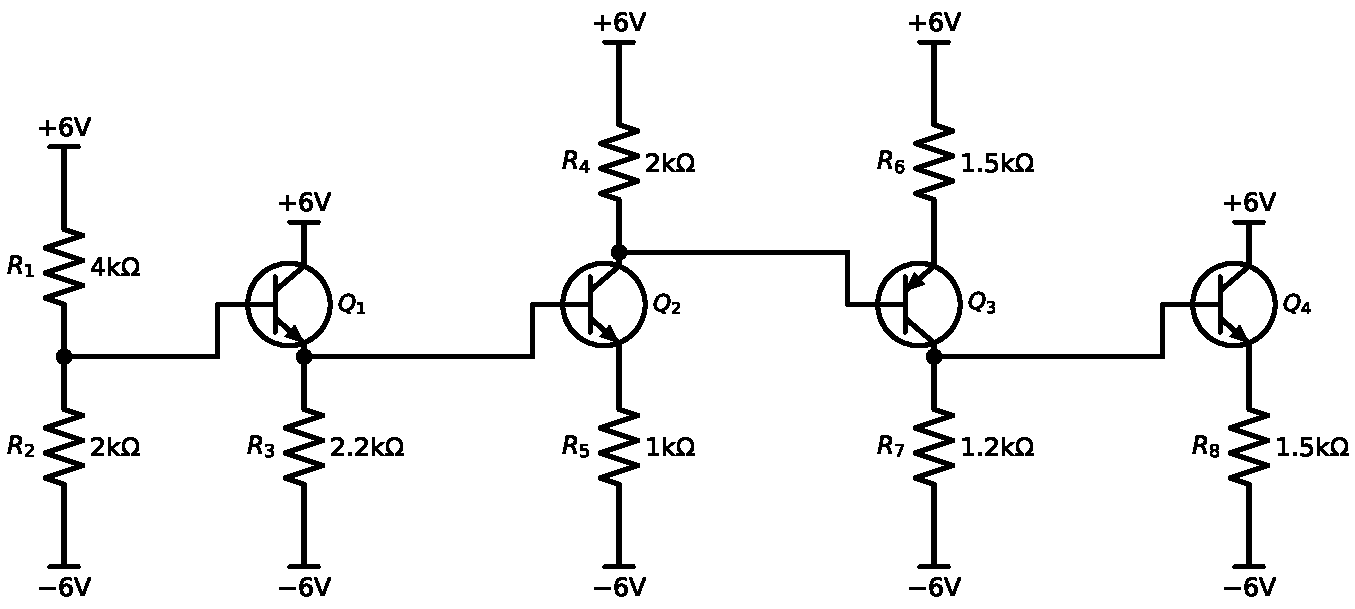
\includegraphics[width=0.9\linewidth,height=6cm,keepaspectratio]{p18_circuit}\end{center}
\solstep{1}{Assumptions}Assume every transistor is in the active region and that every base current is negligible ($I_B\approx0$, tool T1): then $|V_{BE}| = 0.7$\,V, $I_C\approx I_E$, and no current flows into any base, so a base network behaves like a plain resistor divider.
\solstep{2}{Walk through the circuit}\begin{enumerate}[leftmargin=*,itemsep=3pt]
\item No current flows into the base ($I_B$ is negligible), so $V_{B1}$ is set by the divider $R_{1}$--$R_{2}$ between $6$ and $(-6)$ (Lecture-1 tool):\[V_{B1} = -6 + (6 - (-6))\frac{2\,\mathrm{k}}{4\,\mathrm{k} + 2\,\mathrm{k}} = -2\,\mathrm{V}\]
\item $Q_{1}$ is npn and assumed active: $V_{BE} = 0.7$\,V, so $V_{E1} = V_{B1} - 0.7 = -2.7\,\mathrm{V}$.
\item $Q_{2}$ is npn and assumed active: $V_{BE} = 0.7$\,V, so $V_{E2} = V_{E1} - 0.7 = -3.4\,\mathrm{V}$.
\item KCL at the emitter of $Q_{1}$ (base current neglected): \[I_{E1} = \frac{V_{E1} - (-6)}{R_{3}} = 1.5\,\mathrm{m}\mathrm{A}, \qquad I_{C1} \approx I_{E1}\]
\item KCL at the emitter of $Q_{2}$ (base current neglected): \[I_{E2} = \frac{V_{E2} - (-6)}{R_{5}} = 2.6\,\mathrm{m}\mathrm{A}, \qquad I_{C2} \approx I_{E2}\]
\item $Q_{2}$ draws $I_{C2} = 2.6\,\mathrm{m}\mathrm{A}$ from $V_{C2}$ through $R_{4}$: $V_{C2} = 6 - R_{4}\,(I_{C2}) = 6 - 2\,\mathrm{k}\times2.6\,\mathrm{m}\mathrm{A} = 0.8\,\mathrm{V}$.
\item $Q_{3}$ is pnp and assumed active: $V_{BE} = -0.7$\,V, so $V_{E3} = V_{C2} + 0.7 = 1.5\,\mathrm{V}$.
\item KCL at the emitter of $Q_{3}$ (base current neglected): \[I_{E3} = \frac{6 - V_{E3}}{R_{6}} = 3\,\mathrm{m}\mathrm{A}, \qquad I_{C3} \approx I_{E3}\]
\item The current $I_{C3} = 3\,\mathrm{m}\mathrm{A}$ flows from $V_{C3}$ through $R_{7}$: $V_{C3} = (-6) + R_{7}\,(I_{C3}) = -6 + 1.2\,\mathrm{k}\times3\,\mathrm{m}\mathrm{A} = -2.4\,\mathrm{V}$.
\item $Q_{4}$ is npn and assumed active: $V_{BE} = 0.7$\,V, so $V_{E4} = V_{C3} - 0.7 = -3.1\,\mathrm{V}$.
\item KCL at the emitter of $Q_{4}$ (base current neglected): \[I_{E4} = \frac{V_{E4} - (-6)}{R_{8}} = 1.93\,\mathrm{m}\mathrm{A}, \qquad I_{C4} \approx I_{E4}\]
\end{enumerate}

\solstep{3}{Verify the assumptions}\begin{itemize}[leftmargin=*,itemsep=2pt]
\item $I_{B1} = \frac{I_{C1}}{\beta} = 15\,\mu \mathrm{A}$ $\ll$ the $2\,\mathrm{m}\mathrm{A}$ flowing in the base network \checkmark
\item $I_{B2} = \frac{I_{C2}}{\beta} = 26\,\mu \mathrm{A}$ $\ll$ the $1.5\,\mathrm{m}\mathrm{A}$ flowing in the base network \checkmark
\item $I_{B3} = \frac{I_{C3}}{\beta} = 30\,\mu \mathrm{A}$ $\ll$ the $2.6\,\mathrm{m}\mathrm{A}$ flowing in the base network \checkmark
\item $I_{B4} = \frac{I_{C4}}{\beta} = 19.3\,\mu \mathrm{A}$ $\ll$ the $3\,\mathrm{m}\mathrm{A}$ flowing in the base network \checkmark
\item $V_{CE1} = 6 - V_{E1} = 6 - (-2.7) = 8.7\,\mathrm{V}$ $\ge 0.2$\,V $\Rightarrow$ $Q_{1}$ is active \checkmark
\item $V_{CE2} = V_{C2} - V_{E2} = 0.8 - (-3.4) = 4.2\,\mathrm{V}$ $\ge 0.2$\,V $\Rightarrow$ $Q_{2}$ is active \checkmark
\item $V_{EC3} = V_{E3} - V_{C3} = 1.5 - (-2.4) = 3.9\,\mathrm{V}$ $\ge 0.2$\,V $\Rightarrow$ $Q_{3}$ is active \checkmark
\item $V_{CE4} = 6 - V_{E4} = 6 - (-3.1) = 9.1\,\mathrm{V}$ $\ge 0.2$\,V $\Rightarrow$ $Q_{4}$ is active \checkmark
\end{itemize}

\solstep{4}{How good was $I_B\approx 0$?}If we keep the base currents ($I_C=\beta I_B$ with $\beta=100$) and solve the circuit exactly, the currents change only a little:\begin{center}\renewcommand{\arraystretch}{1.35}
\begin{tabular}{cccc}
\toprule
transistor & $I_C$ (with $I_B\approx0$) & $I_C$ (exact) & difference \\
\midrule
$Q_{1}$ & $1.5\,\mathrm{m}\mathrm{A}$ & $1.5\,\mathrm{m}\mathrm{A}$ & $-0.095\%$ \\
$Q_{2}$ & $2.6\,\mathrm{m}\mathrm{A}$ & $2.55\,\mathrm{m}\mathrm{A}$ & $1.8\%$ \\
$Q_{3}$ & $3\,\mathrm{m}\mathrm{A}$ & $2.87\,\mathrm{m}\mathrm{A}$ & $4.4\%$ \\
$Q_{4}$ & $1.93\,\mathrm{m}\mathrm{A}$ & $1.8\,\mathrm{m}\mathrm{A}$ & $7.5\%$ \\
\bottomrule
\end{tabular}\end{center}
 The differences grow along the chain: every base current slightly shifts the collector voltage that biases the next transistor, and $\alpha = \beta/(\beta+1)$ makes each $I_C$ about 1\,\% smaller than its $I_E$. A shift is amplified when the next stage has only a small voltage across its emitter resistor. Hand analysis with $I_B\approx0$ is still the standard first pass.
\begin{ansbox}
$I_{C1} = 1.5\,\mathrm{m}\mathrm{A}$,\quad $I_{C2} = 2.6\,\mathrm{m}\mathrm{A}$,\quad $I_{C3} = 3\,\mathrm{m}\mathrm{A}$,\quad $I_{C4} = 1.93\,\mathrm{m}\mathrm{A}$\\[2pt] all transistors active, all base currents negligible.
\end{ansbox}

\end{document}
